\begin{abstract}
  We consider the problem of inferring and learning latent correlations present in
  multiple noisy matrix-valued datasets using multiset canonical correlation analysis
  (MCCA). We show that MCCA will provably fail to infer the presence of latent
  correlations when the sample size is less than a threshold that is completely specified
  by the dimensionality of the datasets. For the setting where the individual noisy data
  matrices are structured as low-rank-plus-noise, we propose a simple modification of
  MCCA, which we label Informative MCCA (IMCCA).  We show, on both synthetic and real-world
  datasets, that IMCCA reliably infers and learns latent correlations.
\end{abstract}

\section{Introduction}\label{sec:intro}
Multi-modal data fusion is a relevant problem for many emerging machine learning
applications. In these applications, we have access to multiple datasets, possibly
collected using different sensing modalities, each of which describe some feature of the
system. Such datasets have been encountered in machine learning
\cite{hardoon2004canonical, dhillon2011multi ,ahsan2014clustering,chaudhuri2009multi},
medical imaging \cite{correa2010canonical,
  deleus2011functional,zhang2014frequency,guccione2013functional,chen2014removal}, and
multi-temporal hyperspectral imaging \cite{nielsen2002multiset}, to name a few. The goal
is to infer and learn the latent correlations between datasets; dimensionality
reduction algorithms play an important role in this context.

Canonical correlation analysis (CCA) is a classical joint multidimensional dimensionality
reduction algorithm for the two dataset setting \cite{hotelling1936relations}. CCA learns
a linear transformation for each dataset such that the transformed features have maximal
correlation. The extension to the multi-dataset setting is referred to as multiset
canonical correlation analysis (MCCA) and the underlying theory has evolved significantly
over the past few decades \cite{vinograde1950canonical,steel1951minimum,
  horst1961generalized,kettenring1971canonical,nielsen1994analysis}. The five objective
functions (notions of multiset correlation) posed by Kettenring and four constraint
functions on canonical vectors posed by Nielsen give rise to twenty different formulations
of MCCA.

In this paper, we consider the `MAXVAR' formulation as the `most natural 'extension of CCA
to multiple datasets in a sense that we will return to shortly. We begin by deriving the
theoretical solution to MAXVAR assuming known covariance matrices and then consider the
empirical setting where the covariance matrices are unknown and have to be estimated from
a finite number of samples. Substituting the sample covariance matrices into the oracle
MCCA formulation yields the empirical MCCA algorithm. We show that the empirical MCCA
solution can be computed directly by considering the SVD of a block-structured matrix
where the blocks are composed of the pairwise product of the right singular vectors of the
individual data matrices. This leads to the formulation of the informative MCCA (IMCCA)
algorithm, which forms the block-structured matrix using a smaller subset of these
singular vectors corresponding to the `informative components' associated with the latent
low rank matrices. We then show that the IMCCA algorithm can reliably infer and learn
latent correlations in settings where the empirical MCCA algorithm provably cannot.

\section{Multiset Canonical Correlation Analysis}\label{sec:mcca}

Let $y_1\in\complex^{d_1\times 1},\dots,y_m\in\complex^{d_m\times 1}$ model
observations from each of the $m$ datatsets. Define the covariance matrix between all datasets as
\be\ba
&R &&=\E{\left[y_iy_j^H\right]_{i,j=1}^m}= \left[\begin{array}{cccc} R_{11} &
    R_{12} & \cdots & R_{1m}\\ R_{21} & R_{22}& \cdots & R_{2m}\\
  \vdots & \vdots & \ddots & \vdots \\ R_{m1} & R_{m2} & \cdots & R_{mm}\end{array}\right]\\
\ea\ee
and the block diagonal matrix $R_D = \blkdiag(R_{11},R_{22},\dots,R_{mm})$. Both $R$ and $R_D$
are of size $d\times d$ where $d=\sum_{j=1}^md_j$.

The goal of MCCA is to learn canonical coefficient vectors, $x_j\in\complex^{d_j\times 1}$
for $j=1,\dots,m$, such that the canonical variates, $w_j=x_j^Hy_j$, are optimal with
respect to an objective function $J(\cdot)$ and constraint function $h(\cdot)$. Define the
vector of canonical vectors as
$x=\left[x_1^H,\dots,x_m^H\right]^H\in\complex^{d\times 1}$ and the vector of canonical
variates as $w=[w_1,\dots,w_m]^H\in\complex^{m\times 1}$. The covariance matrix of $w$ is
\begin{equation*}
\Phi(x)=\E{ww^H}=\left[\begin{array}{ccc} x_1^HR_{11}x_1 & \dots & x_1^HR_{1m}x_m \\ \vdots
    & \ddots & \vdots \\ x_m^HR_{m1}x_1 & \dots & x_m^HR_{mm}x_m\\ \end{array}\right].
\end{equation*}
Using this notation, the MCCA optimization problem is
\begin{equation}\label{eq:chpt10:opt_prob}
\begin{aligned}
&\underset{x}{\mathop{\rm optimize}} && J(\Phi(x))\\
&\text{subject to} && h(x,R).\\
\end{aligned}
\end{equation}
In \cite{kettenring1971canonical}, Kettenring summarizes five commonly used objective
functions and Nielson summarizes four commonly used constraint functions in
\cite{nielsen1994analysis}. In this paper we consider the maximum variance (MAXVAR)
objective function, which seeks to maximize the largest eigenvalue of $\Phi(x)$, and the
constraint functions $x_j^HR_{jj}x_j = 1,\, j=1,\dots,m$,
which require the canonical variates to be unit norm. Therefore, the MCCA optimization
problem considered herein is
\begin{equation}\label{eq:chpt10:opt_prob2}
\begin{aligned}
&\argmax_x && \lambda_1\left(\Phi(x)\right)\\
&\text{subject to} && x_j^HR_{jj}x_j = 1,\, j=1,\dots,m,\\
\end{aligned}
\end{equation}
where $\lambda_1(M)$ is the largest eigenvalue of a matrix $M$.

\subsection{Solution to MAXVAR}
We rewrite the MAXVAR optimization problem in (\ref{eq:chpt10:opt_prob2}) as
\begin{equation}\label{eq:chpt10:maxvar}
\begin{aligned}
&\argmax_{x}&&\lambda\\
&\text{subject to} &&x_i^HR_{ii}x_i  = 1\,\,,1\leq i\leq m,\\
&&&\Phi(x) a = \lambda a, \,\,\,\,\,a^Ha=1.\\
\end{aligned}
\end{equation}
Writing $\Phi(x) = X^H R X$, where $X=\blkdiag(x_1,\dots,x_m)$, and making the
transformation $\widetilde{a}=R_D^{1/2}Xa$, (\ref{eq:chpt10:maxvar}) becomes
\begin{equation}\label{eq:chpt10:maxvar2}
\begin{aligned}
&\argmax_{\widetilde{a}}&&\lambda\\
&\text{subject to}&& \widetilde{a}^HR_D^{-1/2}RR_D^{-1/2}\widetilde{a} = \lambda,\,\,\,\,\, \widetilde{a}^H\widetilde{a}=1.\\
\end{aligned}
\end{equation}
The solution to this formulation is immediately solved by examining the matrix
\beq\label{eq:chpt10:rmcca}
\Rmcca =R_D^{-1/2}RR_D^{-1/2}.
\eeq
The largest eigenvalue of $\Rmcca$ is exactly $\lambda$ in (\ref{eq:chpt10:maxvar2}) and
$\widetilde{a}$ is exactly the corresponding eigenvector. To recover the canonical
vectors, we simply invert our original transformation to obtain
\beq\label{eq:chpt10:can_vect}
x_j = \frac{R_{jj}^{-1/2}\widetilde{a}_j}{\|\widetilde{a}_j\|},
\eeq
where $\widetilde{a}_j\in\complex^{d_i}$ is the component of $\widetilde{a}$ corresponding
to dataset $j$. We may obtain higher order canonical vector and canonical correlation
pairs by taking successive eigenvalue-eigenvector pairs of $\Rmcca$. We denote the $i$th
order canonical vector with the superscript $x_j^{(i)}$ corresponding to $\lambda_i$.

Examining (\ref{eq:chpt10:rmcca}), we see that if all of the datasets are uncorrelated
($R_{ij}=0$), $\Rmcca=I_d$ and all eigenvalues of $\Rmcca$ are equal to 1. This motivates the use of the statistic
\beq\label{eq:chpt10:mcca_stat}
\lambda_i -1,
\eeq
to infer the presence of latent correlations in multiple datasets.

\subsection{Empirical MAXVAR}
In  a practical setting, the covariance matrices used to form $R$ and $R_D$ needed
for $\Rmcca$ in (\ref{eq:chpt10:rmcca}) are unknown and hence have to be learned from
training data. We stack the $n$ observations from each dataset to form the $m$ training
data matrices 
\beq\label{eq:chpt10:data_matrices}
Y_j=\left[y_j^{(1)},\dots
  y_j^{(n)}\right]\in\complex^{d_j\times n}, j=1,\dots,m.
\eeq
Substituting the sample covariance matrices (which are the maximum-likelihood estimates under a Gaussian prior),
$\widehat{R}_{ij}=\frac{1}{n}Y_iY_j^H$, into (\ref{eq:chpt10:rmcca}) yields the plug-in estimate
$\Rmccahat$. Henceforth, we shall label canonical vectors obtained from an  analysis of the eigen-structure of $\Rmccahat$ as empirical
MAXVAR or empircal MCCA.

To explore the structure of $\Rmccahat$, denote the SVD of each training dataset as
$Y_j=\widehat{U}_j\widehat{\Sigma}_j\widehat{V}_j^H$ and form the block matrices
$\widehat{U}=\blkdiag(\widehat{U}_1,\dots,\widehat{U}_m)\in\complex^{d\times d}$,
$\widehat{\Sigma}=\blkdiag(\widehat{\Sigma}_1,\dots,\widehat{\Sigma}_m)\in\complex^{d\times nm}$, and
$\widehat{V}=[\widehat{V}_1,\dots,\widehat{V}_m]\in\complex^{n\times nm}$. With these definitions, we form
$\widehat{R}=\widehat{U}\widehat{\Sigma} \widehat{V}^H\widehat{V}\widehat{\Sigma}^H\widehat{U}^H$ and $\widehat{R}_D=\widehat{U}\widehat{\Sigma}\widehat{\Sigma}^H\widehat{U}^H$. After some straightforward
algebraic manipulations, we note that
\begin{equation}\label{eq:chpt10:rmccahat}
\begin{aligned}
&\Rmccahat=\widehat{R}_D^{-1/2}\widehat{R}\widehat{R}_D^{-1/2}=\widetilde{U}\widetilde{V}^H\widetilde{V}\widetilde{U}^H,\\
%&&&=\left(\widehat{U}\widehat{\Sigma}\widehat{\Sigma}^H\widehat{U}^H\right)^{-1/2}\left(\widehat{U}\widehat{\Sigma} \widehat{V}^H\widehat{V}\widehat{\Sigma}^H \widehat{U}^H\right)\left(\widehat{U}\widehat{\Sigma}\widehat{\Sigma}^H\widehat{U}^H\right)^{-1/2},\\
%&&&=U(\Sigma\Sigma^H)^{-1/2}U^HU\Sigma V^HV\Sigma^HU^HU(\Sigma\Sigma^H)^{-1/2}U^H\\
%&&& = U(\Sigma\Sigma^H)^{-1/2}\Sigma V^HV\Sigma^H(\Sigma\Sigma^H)^{-1/2}U^H\\
%&&&=\widetilde{U}\widetilde{V}^H\widetilde{V}\widetilde{U}^H,
\end{aligned}
\end{equation}
where 
{\small{
\be\ba
&{\small{\widetilde{U}=\blkdiag(\widehat{U}_1(:,1:\min(n,d_1)),\dots,\widehat{U}_m(:,1:\min(n,d_m)))}}\\
&\widetilde{V}=[\widehat{V}_1(:,1:\min(n,d_1)),\dots,\widehat{V}_m(:,1:\min(n,d_m))].\\
\ea\ee
}}
From this, we see that the eigenvalues of $\Rmccahat$ are exactly the eigenvalues of
$\widetilde{V}^H\widetilde{V}$. Let $\widehat{\lambda}_i$ be the eigenvalues of
$\Rmccahat$. Thus the statistic
\beq\label{eq:chpt10:emp_mcca_stat}
\widehat{\lambda}_i-1,
\eeq
might be used to infer the presence of latent correlations. Note that (\ref{eq:chpt10:emp_mcca_stat}) is the plug-in estimate of the statistic in (\ref{eq:chpt10:mcca_stat}).

Consider the special setting where we have exactly two datasets. Then it can be seen that empirical MAXVAR reduces to the standard empirical CCA
problem which involves an eigen-analysis of the matrix
\beq\label{eq:chpt10:R_cca}
\widehat{R}_{\text{cca}} =
\left[\begin{array}{c}\widehat{V}_1^H\\\widehat{V}_2^H\end{array}\right]\left[\begin{array}{cc}\widehat{V}_1 &
    \widehat{V}_2\end{array}\right] = \left[\begin{array}{cc}I_{d_1} &
    \widehat{V}_1^H\widehat{V}_2\\ \widehat{V}_2^H\widehat{V}_1 & I_{d_2}\end{array}\right].
\eeq
Bach and Jordan \cite{bach2003kernel}, note that the
eigenvalues of $\widehat{R}_{\text{cca}}$ come in pairs,
$\left\{1+\lambda_i,1-\lambda_i,\right\}$. 
Thus in the CCA setting, maximizing the largest eigenvalue of
$R_{\text{cca}}$ as in (\ref{eq:chpt10:opt_prob2}) is equivalent to minimizing the smallest eigenvalues of
$R_{\text{cca}}$. The formulation that leads to minimizing the smallest eigenvalue is referred to as MINVAR. For the multiple datasets setting, the MINVAR formulation involves
minimizing the eigenvalues of $\Rmccahat$. Bach and Jordan \cite{bach2003kernel} also
point out
that the minimum eigenvalue of $\Rmccahat$ is always bounded between zero and one while
the maximum eigenvalue grows with added datasets. In the following section, we willl establish conditions that establish when the the MAXVAR test statistic  in (\ref{eq:chpt10:emp_mcca_stat}) will provably fail to infer the presence of latent correlations. We shall also provide conditions when the analogous MINVAR test statistc fails to infer latent correlations.


\section{New Theoretical Results}\label{sec:theory}

A key result in two-dataset empirical CCA is that when the number of samples is less than
the combined dimension of the datasets ($n<d_1+d_2$) then the largest eigenvalue of
$R_{\text{cca}}$ is deterministically equal to $2$ \cite{pezeshki2004empirical}, regardless of
whether an underlying correlation actually exists between the datasets. We now prove an
analogous statement for the MAXVAR formulation of MCCA for the setting where $m >2$.


\begin{Th}\label{th:maxvar}
Let $m>2$ be the number of datasets to use in MCCA. If $2n<\min_{i\neq j\neq
  k}(d_i+d_j+d_k)$ then the largest eigenvalue of $\Rmccahat$ is equal to $m$.
\end{Th}

 In high-dimensional settings, because of computational complexity considerations, it is often prudent to learn correlations only when they are detected  to be statistically significant. Theorem \ref{th:maxvar} establishes conditions when the empirical MAXVAR test statistic in (\ref{eq:chpt10:emp_mcca_stat}) will provably fail to infer the presence of correlations despite the presence of correlations.  We now establish a similar result for the MINVAR test statistic.

\begin{Th}\label{th:minvar}
If $n<\sum_{i=1}^md_i$ then the smallest eigenvalue of $\Rmcca$ is zero.
\end{Th}

Comparing statements of Theorems \ref{th:maxvar} and \ref{th:minvar} shows that there is a sample complexity gap for the failure of MINVAR and MAXVAR that we believe is loose. Tighteting it remains an open problem.

\section{New Algorithm: Informative MCCA}\label{sec:imcca}

Empirical MCCA places no model on the observations and so we simply stack the observations
in data matrices as in (\ref{eq:chpt10:data_matrices}). We now consider a setting where the
observations of each dataset have latent low-rank plus noise structure. We denote the
$i$th observation from the $j$th dataset as $y_j^{(i)}$ as in
(\ref{eq:chpt10:data_matrices}) and model them as 
\beq\label{eq:chpt10:mcca_data_model}
y_j^{(i)} = U_js_j^{(i)} + z_j^{(i)},
\eeq
where  $U_j^HU_j=I_{k_j}$ model the low-rank signal subspace of each dataset and
$z_j^{(i)}\simiid\mathcal{CN}(0,I_{d_j})$ model the noise. Furthermore, assume that signals are
modeled as
\be
s_j^{(i)}\simiid\mathcal{CN}(0,\Theta_j)\\
\ee
where
$\Theta_j=\diag\left(\left(\theta_j^{(1)}\right)^2,\dots,\left(\theta_j^{(k_j)}\right)^2\right)$. Assume
that for all $j$ and $i$, $z_j^{(i)}$ are mutually independent and independent
from all $s_j^{(i)}$. Finally, assume that the signal covariance is modeled as
\be
\E{s_j s_\ell^{H}} \defeq K_{j\ell} = \Theta_j^{1/2}P_{j\ell}\Theta_\ell^{1/2}
\ee
where the entries of $P_{j\ell}$ are between $-1$ and $1$ and represent the correlation
between the entries of $s_j$ and $s_\ell$.  Under this model, the covariance matrices are
\beq\label{eq:chpt10:mcca_true_scm}\ba
&\E{y_jy_j^H} = U_j\Theta_jU_j^H+I_{d_j} \defeq R_{jj}\\
&\E{y_jy_\ell^H} = U_jK_{j\ell}U_\ell^H \defeq R_{j\ell}.\\
\ea\eeq

\subsection{IMCCA}

Empirical MCCA examines the eigen-decomposition of the matrix $\Rmccahat =
\widetilde{U}\widetilde{V}^H\widetilde{V}\widetilde{U}^H$. This matrix uses the entire
spectrum of all the datasets. Under the low-rank
signal-plus-noise model, this is incorrect as each dataset is low-rank.

Motivated by this observation from the low-rank data model in
(\ref{eq:chpt10:mcca_data_model}), we expect the principal components (or top few singular
vectors) of the SVD of these matrices to be `informative' (\textit{i.e.}, correlated with
the latent vectors in (\ref{eq:chpt10:mcca_data_model}). Thus our idea is to form the
matrix $\Rmccahat$ from just the principal `informative' singular vectors instead of all
the singular vectors. This leads to our so-called informative version of MAXVAR.

Let $\widehat{k}_j$ be estimates of the number of the latent rank of the low-rank matrix in (\ref{eq:chpt10:mcca_data_model})  or equivalently, of the number of principal components used from each dataset. We then form the matrices
\be
\Ucir_j = \widehat{U}_j\left(:,1:\widehat{k}_j\right),\,\Vcir_j = \widehat{V}_j\left(:,1:\widehat{k}_j\right).
\ee
Let
\be
\Ucir = \blkdiag(\Ucir_1,\dots,\Ucir_m),\,\,\,\,\Vcir =
\left[\Vcir_1,\dots \Vcir_m\right],
\ee
and define the informative MAXVAR (IMCCA) matrix as
\beq\label{eq:chpt10:rimcca}
\Rmccatil = \Ucir\Vcir^H\Vcir\Ucir^H.
\eeq
Denote the eigenvalues of this IMCCA matrix by $\widetilde{\lambda}_i$. As in,
(\ref{eq:chpt10:mcca_stat}) we propose using
\beq\label{eq:chpt10:imcca_stat}
\widetilde{\lambda}_i -1,
\eeq
as a test statistic to infer the presence of latent correlations. Once the correlations
are detected then they can be learned. The IMCCA canonical vector estimate is found by
substituting the eigenvectors of $\Rmccatil$ in (\ref{eq:chpt10:can_vect}) along with the
covariance matrix estimates found by substituting parameter estimates in
(\ref{eq:chpt10:mcca_true_scm}). 

\section{Results}\label{sec:results}
We note that the statistic in (\ref{eq:chpt10:imcca_stat}) is computationally much more tractable to compute than (\ref{eq:chpt10:mcca_stat}) when $\max_{j} \widehat{k}_{j} \ll d_j$.  In what follows, we will show that the resulting test statistic and the associated learned vectors are more informative as well.
\subsection{Numerical Simulations}\label{sec:num_sims}

To validate Theorem \ref{th:maxvar} and to compare the ability of the empirical MCCA
and IMCCA algorithms to infer the presence of correlations, we consider a rank-1 setting in (\ref{eq:chpt10:mcca_data_model}).  We set $d_1 =d_2=d_3=150$, $k_1=k_2=k_3=1$, and
$P_{12}=P_{13}=P_{23}=0.9$. We then sweep over $n$ and
$\theta=\theta_1=\theta_2=\theta_3$. For each value of $n$ and $\theta$, we generate data
matrices from data modeled in (\ref{eq:chpt10:mcca_data_model}), form $\Rmccahat$ in
(\ref{eq:chpt10:rmccahat}) or $\Rmccatil$ in (\ref{eq:chpt10:rimcca}), and compute its
largest eigenvalue. We then generate $\Rmccahat$ (or $\Rmccatil$) from purely noise only
matrices where the noise is modeled exactly as in (\ref{eq:chpt10:mcca_data_model}). We
repeat this for 500 trials to obtain 500 eigenvalues from signal bearing $\Rmccahat$ (or
$\Rmccatil$) and 500 eigenvalues from noise only $\Rmccahat$ (or $\Rmccatil$). Figure
\ref{fig:chpt10:heatmap} plots the Kolmorgorv-Smirnov (KS) statistic (significance value
of 0.05) used to test if the distributions between the signal-bearing and noise-only
eigenvalues are statistically different. A value of 1 represents the distributions are
statistically different while a value of 0 represents the distributions are identical. For
IMCCA, we set $\widehat{k}_1=\widehat{k}_2=\widehat{k}_3=1$.

\begin{figure}
  \begin{center}
    \subfigure[Empirical MCCA]{
      \label{fig:chpt10:heatmap_mcca}
      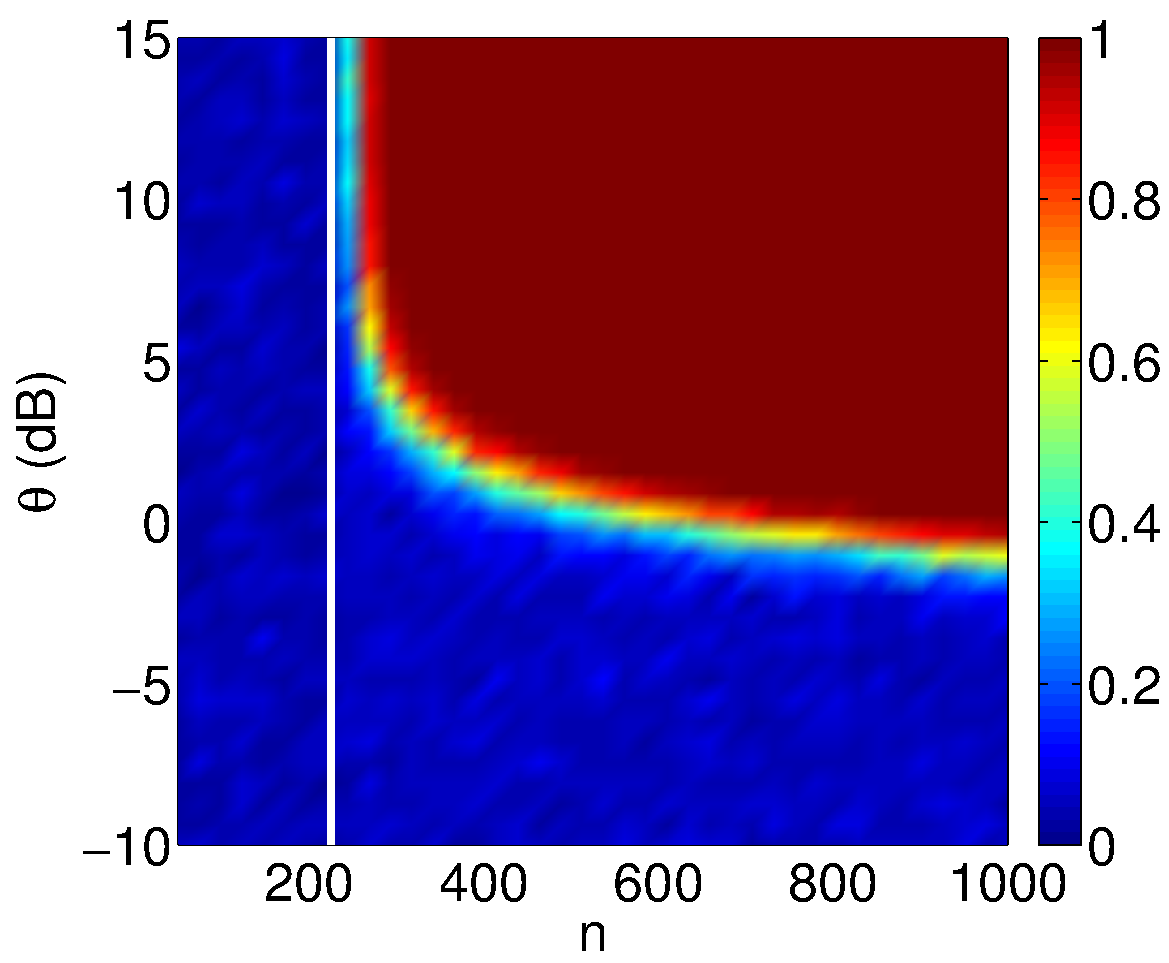
\includegraphics[width=0.22\textwidth]{chpt10_mcca/figs/mcca_pt.pdf}
    }
    \subfigure[IMCCA]{
      \label{fig:chpt10:heatmap_imcca}
      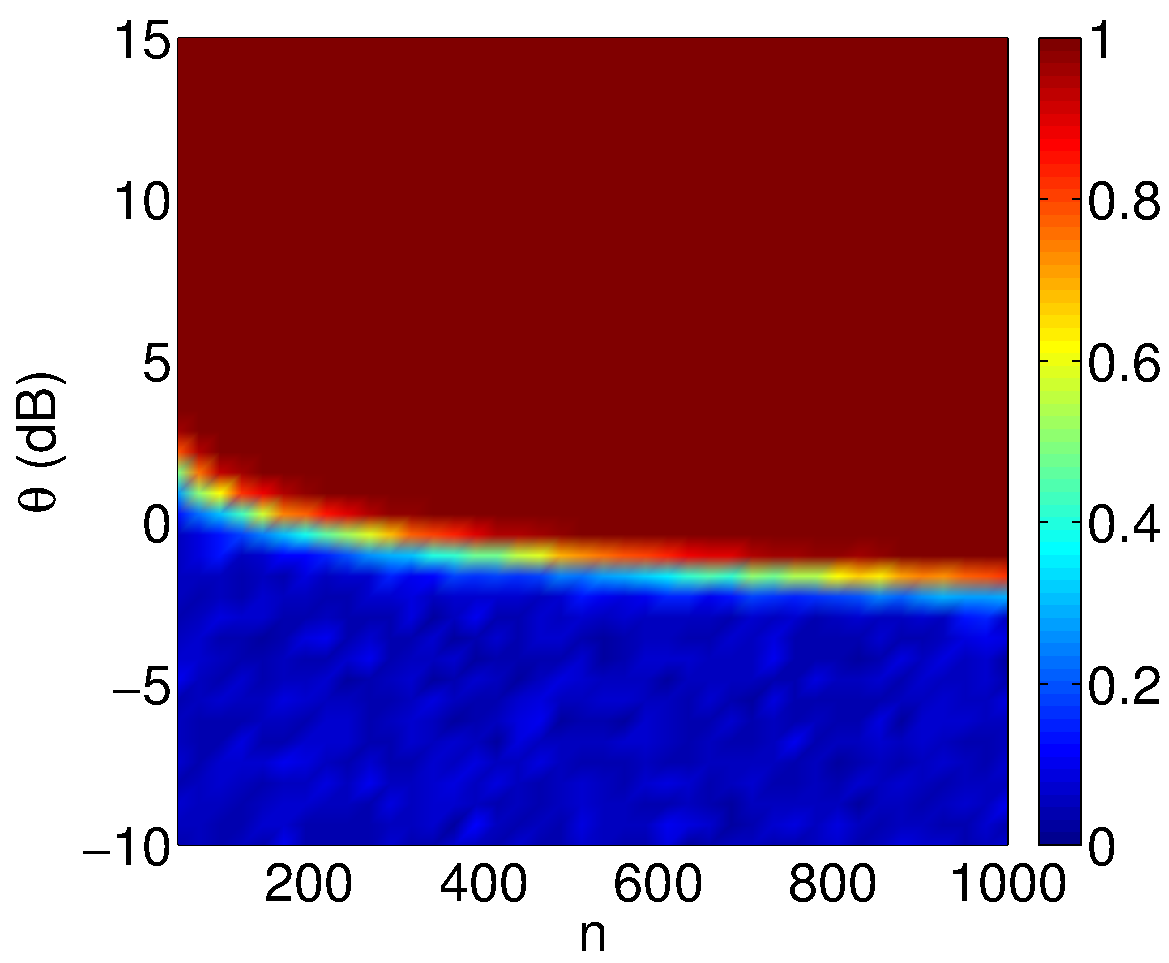
\includegraphics[width=0.22\textwidth]{chpt10_mcca/figs/imcca_pt.pdf}
    }
    \caption{Heatmaps for detection of a correlated signal for a rank-1 setting of
      $d_1=d_2=d_3=150$, $k_1=k_2=k_3=1$, and $P_{12}=P_{13}=P_{23}=0.9$. We generate data
      from (\ref{eq:chpt10:mcca_data_model}) for various choices of $n$ and
      $\theta=\theta_1=\theta_2=\theta_3$ and when the data in
      (\ref{eq:chpt10:mcca_data_model}) is noise only. We then take the largest eigenvalue
      of $\Rmccahat$ in (\ref{eq:chpt10:rmccahat}) and $\Rmccatil$ (\ref{eq:chpt10:rimcca})
      for both the signal and noise only cases and repeat for 500 trials. We plot the
      Kolmorgov-Smirnov test statistic between the eigenvalue distributions of the signal
      and noise only cases. (a) Results for empirical MCCA. The white line is minimum
      number of samples needed for non-deterministic eigenvalues as predicted by Theorem
      \ref{th:maxvar}. When we have fewer samples than this limit, the empirical MCCA test statistic cannot
      infer the presence of the correlated signal. (b) Results for IMCCA. The IMCCA test statistic is able
      to infer the presence of the correlated signal in the small-sample regime.}
    \label{fig:chpt10:heatmap}
  \end{center}
\end{figure}

Ideally, we wish the distributions of the top eigenvalues of signal bearing and noise-only
matrices to be different in all parameter regimes. However, as evident in Figure
\ref{fig:chpt10:heatmap_mcca}, in the small-sample, high-dimensional regime, the
distributions of the largest eigenvalue used by empirical MCCA are identical whether the
datasets have latent correlations or not. This is undesirable and verifies Theorem
\ref{th:maxvar}. For our simulation parameters this theorem states that when $n<225$ the
maximum eigenvalue is deterministic, which is verified by the simulation. However, IMCCA
is able to overcome this undesirable performance loss by first trimming data matrices to
only include the number of signal components present in the data. From this numerical
example, we see that our new algorithm, IMCCA, can reliably infer the presence of
correlations in multiple datasets in the low-sample, high-dimensionality regime.

\subsection{Real World Video Example}\label{sec:real}

To verify the effectiveness of IMCCA for real world applications and to showcase the
extreme sub-optimality of empirical MCCA, we setup a controlled experiment consisting of
four stationary flashing lights and three stationary iPhone cameras. Figure
\ref{fig:chpt10:mcca_sources} manually identifies each source in each camera view by
drawing a colored box around it. The left camera can see a flashing laptop screen (L1), a
flashing phone light (PH1), and a flashing tablet screen (T1). The middle camera has only
one source, the flashing tablet screen (T1). The right camera can see the flashing tablet
screen (T1), the flashing laptop screen (L1) via an external monitor, and a flashing
police light (PL1). Based on our setup, all cameras share the T1 source, while the left
and right views share the L1 source. The left and right views also each have an
independent source in their view.

\begin{figure*}
  \begin{center}
    \subfigure[Left Camera]{
      \label{fig:chpt10:mcca_man_left}
      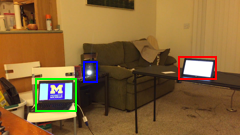
\includegraphics[width=0.3\textwidth]{chpt10_mcca/figs/mcca_left_man.png}
    }
    \subfigure[Middle Camera]{
      \label{fig:chpt10:mcca_man_mid}
      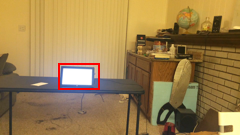
\includegraphics[width=0.3\textwidth]{chpt10_mcca/figs/mcca_mid_man.png}
    }
    \subfigure[Right Camera]{
      \label{fig:chpt10:mcca_man_right}
      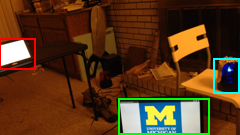
\includegraphics[width=0.3\textwidth]{chpt10_mcca/figs/mcca_right_man.png}
    }
    \caption{Manual identification of each source in each camera. All three sources share
      a common flashing tablet, outlined in red. The left and right camera views share a
      common flashing laptop screen, outlined in green. The left camera has an independent
      flashing phone light, outlined in dark blue. The right camera has an independent
      flashing police light, outlined in cyan.}
    \label{fig:chpt10:mcca_sources}
  \end{center}
\end{figure*}


To synchronize the cameras we used the RecoLive MultiCam iPhone app
\footnote{http://recolive.com/en/}. After turning on all light sources, we recorded 20
seconds of video at 30 frames per second. The resolutions of the iPhone's cameras were all
$1920\times 1080$ pixels. To post-process the video data, we first converted the video
streams to grayscale and then downsampled each spatial dimension by a factor of 8,
resulting in a resolution of $240\times 135$. We then vectorized each image and stacked
the 600 frames into data matrices, all of dimension $32400 \times 600$.

We run empirical MCCA and IMCCA after every frame. Specifically, for frame $\ell$, we
construct the $32400\times \ell$ submatrices $Y_{\text{left}}^{\ell}$,
$Y_{\text{middle}}^{\ell}$, and $Y_{\text{right}}^{\ell}$ by taking the matrix of the
first $\ell$ vectorized frames in each view and then subtracting the mean of the
resulting submatrix. We then use these resulting submatrices as inputs to empirical MCCA
and IMCCA in equations (\ref{eq:chpt10:rmccahat}) and (\ref{eq:chpt10:rimcca}),
respectively. Using our knowledge of the number of sources in each camera, we set
$\widehat{k}_{\text{left}}=3$, $\widehat{k}_{\text{middle}}=1$, and
$\widehat{k}_{\text{right}}=3$. Figure \ref{fig:chpt10:mcca_corrs} plots the top 3
correlation statistics returned by empirical MCCA and IMCCA, as defined in
(\ref{eq:chpt10:emp_mcca_stat}) and (\ref{eq:chpt10:imcca_stat}), respectively. As
expected due to the extreme sample deficient regime, the empirical MCCA statistics are
equal to $2=m-1$, which incorrectly identifies the top three canonical vectors as being
perfectly correlated. However, the IMCCA statistic correctly identifies two correlations
that exist. The third correlation statistic returned by IMCCA is essentially zero.

\begin{figure}
  \begin{center}
    \subfigure[MCCA]{
      \label{fig:chpt10:mcca_mid_u1}
      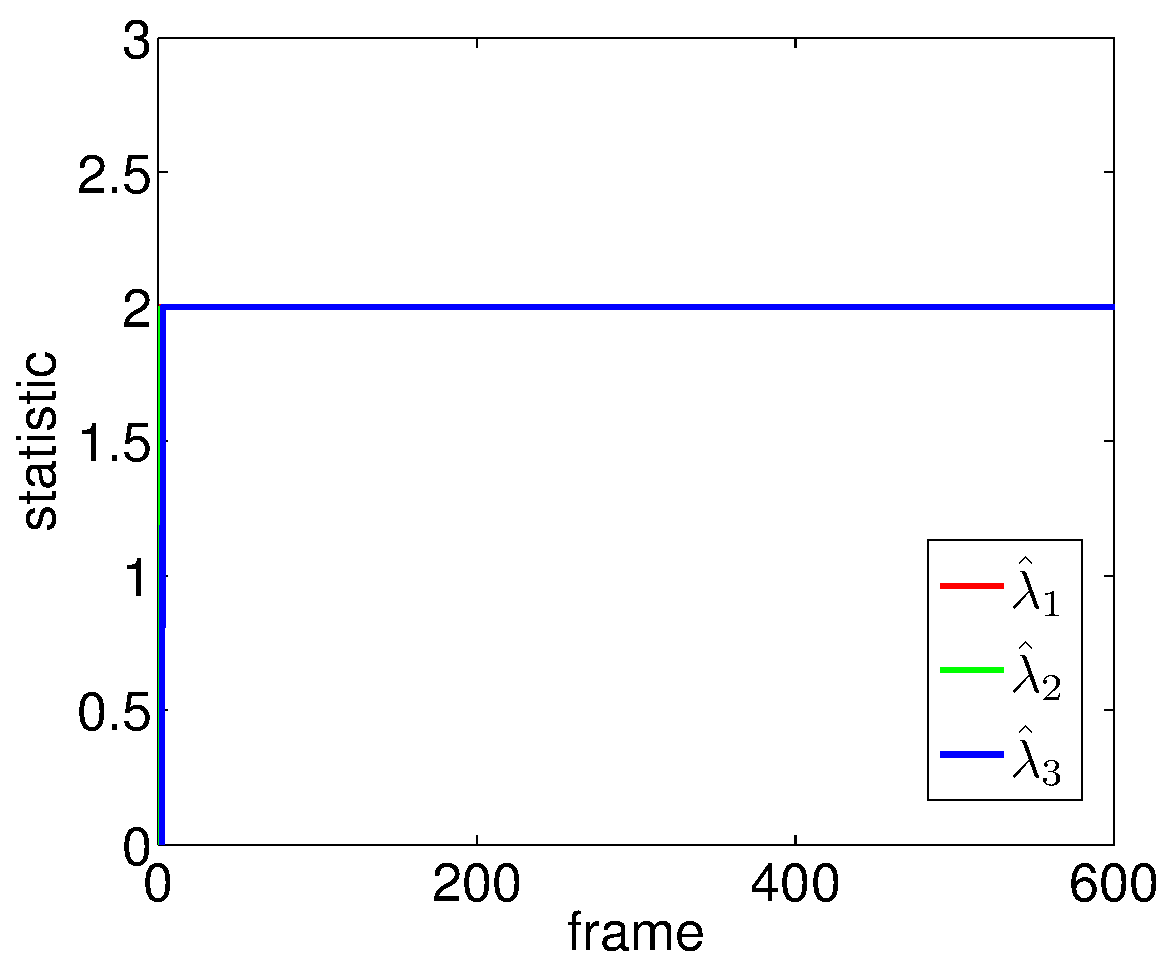
\includegraphics[width=0.22\textwidth]{chpt10_mcca/figs/mcca_corrs.pdf}
    }
    \subfigure[IMCCA]{
      \label{fig:chpt10:mcca_mid_overlay}
      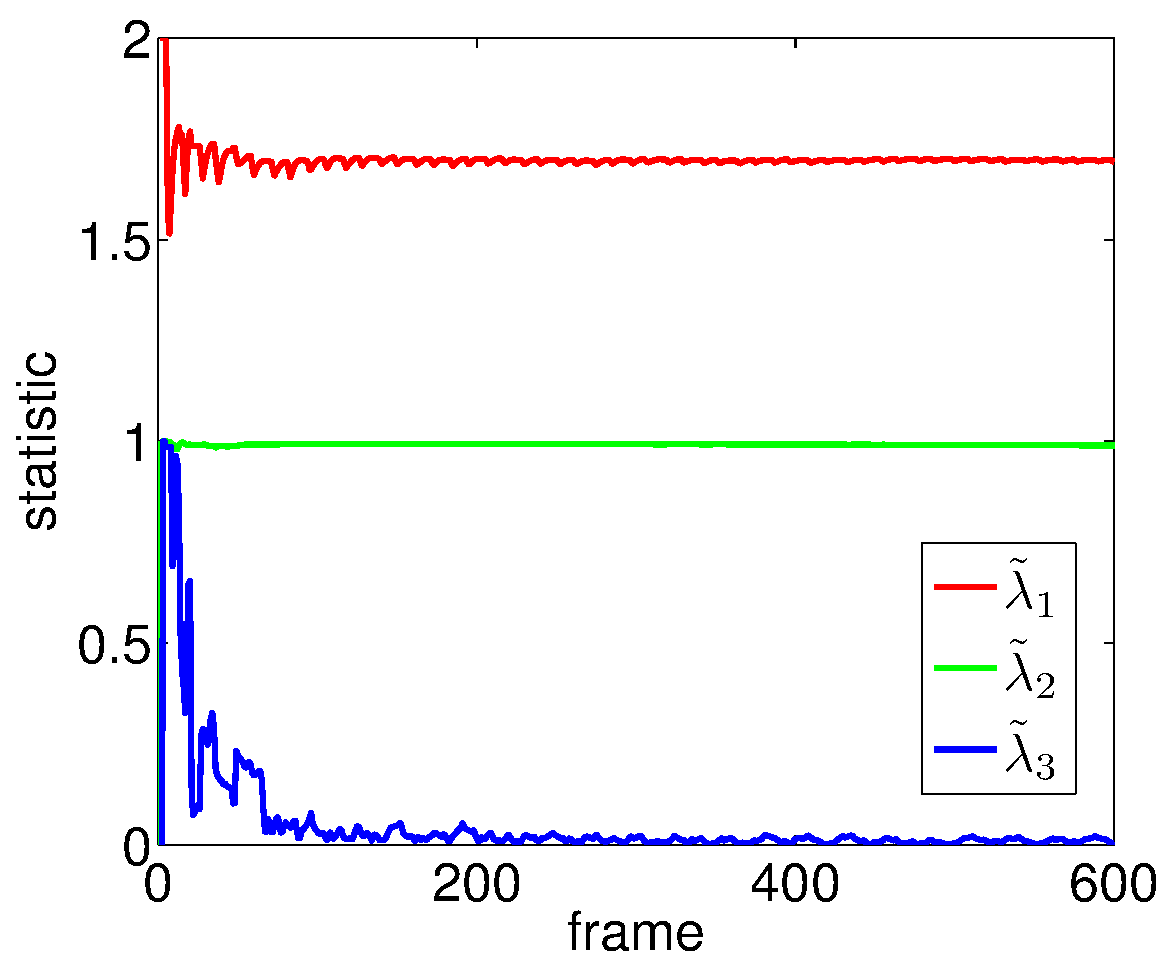
\includegraphics[width=0.22\textwidth]{chpt10_mcca/figs/imcca_corrs.pdf}
    }
    \caption{Top 3 correlation statistics returned over the 600 frames of video. (a)
      Empirical MCCA statistic as defined in (\ref{eq:chpt10:emp_mcca_stat}). (b) IMCCA
      statistic as defined in (\ref{eq:chpt10:imcca_stat}).}
    \label{fig:chpt10:mcca_corrs}
  \end{center}
\end{figure}

Figure \ref{fig:chpt10:mcca_cca_vects} plots the canonical vectors associated with the top
two correlation statistics for empirical MCCA and IMCCA as computed by
(\ref{eq:chpt10:can_vect}). The learned MCCA canonical vectors appear extremely random
and noisy while the learned IMCCA canonical vectors correctly identify the two sources of
correlation in our video. We note that there is not a second IMCCA canonical vector for
the middle camera because there is only one light source in the view. IMCCA correctly
identifies that one source of correlation appears in all three views and that one source
of correlation appears in only the left and right views. Please see the supplementary
material for a video overlaying these canonical vectors onto the original scene.


%\begin{figure}
%  \begin{center}
%    \subfigure[MCCA Left Camera]{
%      \label{fig:chpt10:mcca_cca_left}
%      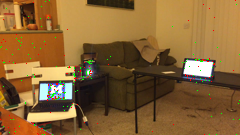
\includegraphics[width=0.3\textwidth]{chpt10_mcca/figs/mcca_left_cca.png}
%    }
%    \subfigure[MCCA Middle Camera]{
%      \label{fig:chpt10:mcca_cca_mid}
%      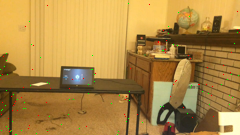
\includegraphics[width=0.3\textwidth]{chpt10_mcca/figs/mcca_mid_cca.png}
%    }
%    \subfigure[MCCA Right Camera]{
%      \label{fig:chpt10:mcca_cca_right}
%      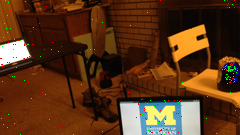
\includegraphics[width=0.3\textwidth]{chpt10_mcca/figs/mcca_right_cca.png}
%    }
%    \subfigure[IMCCA Left Camera]{
%      \label{fig:chpt10:mcca_icca_left}
%      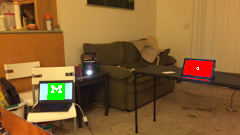
\includegraphics[width=0.3\textwidth]{chpt10_mcca/figs/mcca_left_icca.png}
%    }
%    \subfigure[IMCCA Middle Camera]{
%      \label{fig:chpt10:mcca_icca_mid}
%      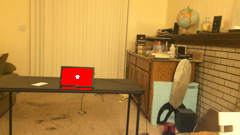
\includegraphics[width=0.3\textwidth]{chpt10_mcca/figs/mcca_mid_icca.png}
%    }
%    \subfigure[IMCCA Right Camera]{
%      \label{fig:chpt10:mcca_icca_right}
%      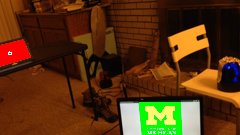
\includegraphics[width=0.3\textwidth]{chpt10_mcca/figs/mcca_right_icca.png}
%    }
%    \caption{Top 2 thresholded canonical vectors overlayed onto the original scene. The
%      red pixels are the pixels corresponding to the largest correlation and the green
%      pixels correspond to the pixels with the second largest correlation. The top row
%      shows the MCCA canonical vectors; the bottom row shows the IMCCA canonical
%      vectors. Since we are in the sample deficient regime, MCCA returns random pixels as
%      the canonical vectors are random. IMCCA correctly identifies the shared light in all
%      three views with the red pixels and the shared laptop light in the left and right
%      views with the green pixels.}
%    \label{fig:chpt10:mcca_cca_vects}
%  \end{center}
%\end{figure}

\begin{figure*}
  \begin{center}
    \subfigure[MCCA Left $x^{(1)}$]{
      \label{fig:chpt10:mcca_cca_left1}
      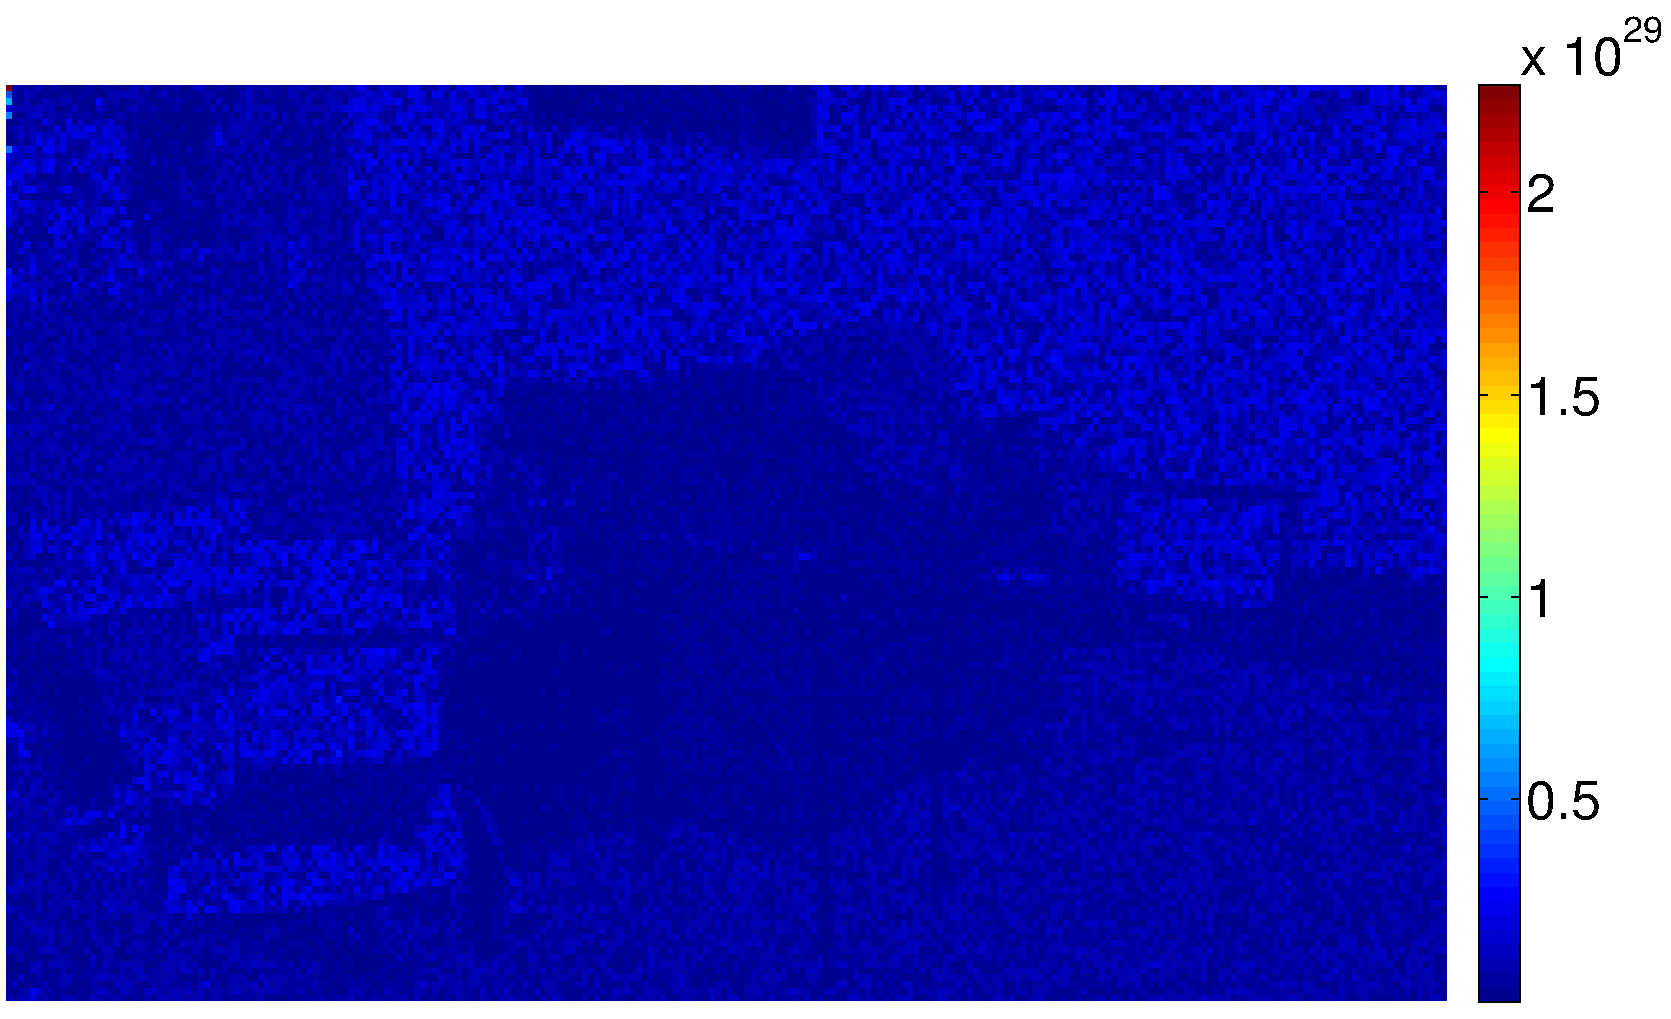
\includegraphics[width=0.3\textwidth]{chpt10_mcca/figs/mcca_ul1.pdf}
    }
    \subfigure[MCCA Middle $x^{(1)}$]{
      \label{fig:chpt10:mcca_cca_mid1}
      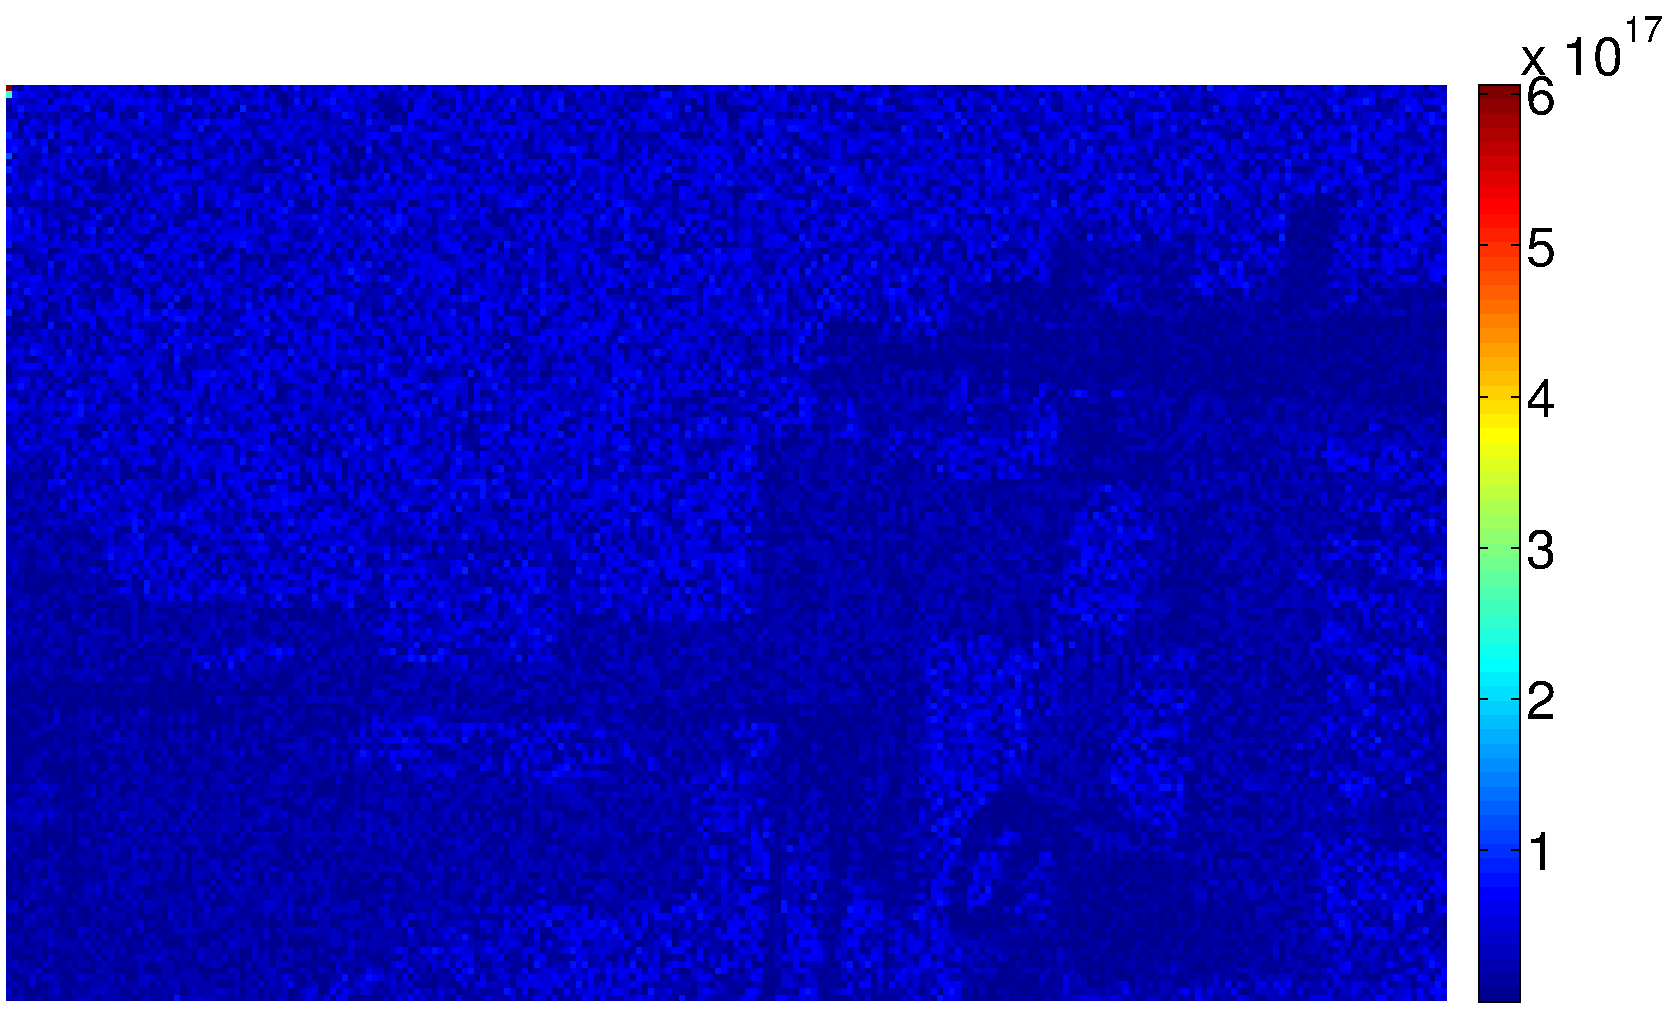
\includegraphics[width=0.3\textwidth]{chpt10_mcca/figs/mcca_um1.pdf}
    }
    \subfigure[MCCA Right $x^{(1)}$]{
      \label{fig:chpt10:mcca_cca_right1}
      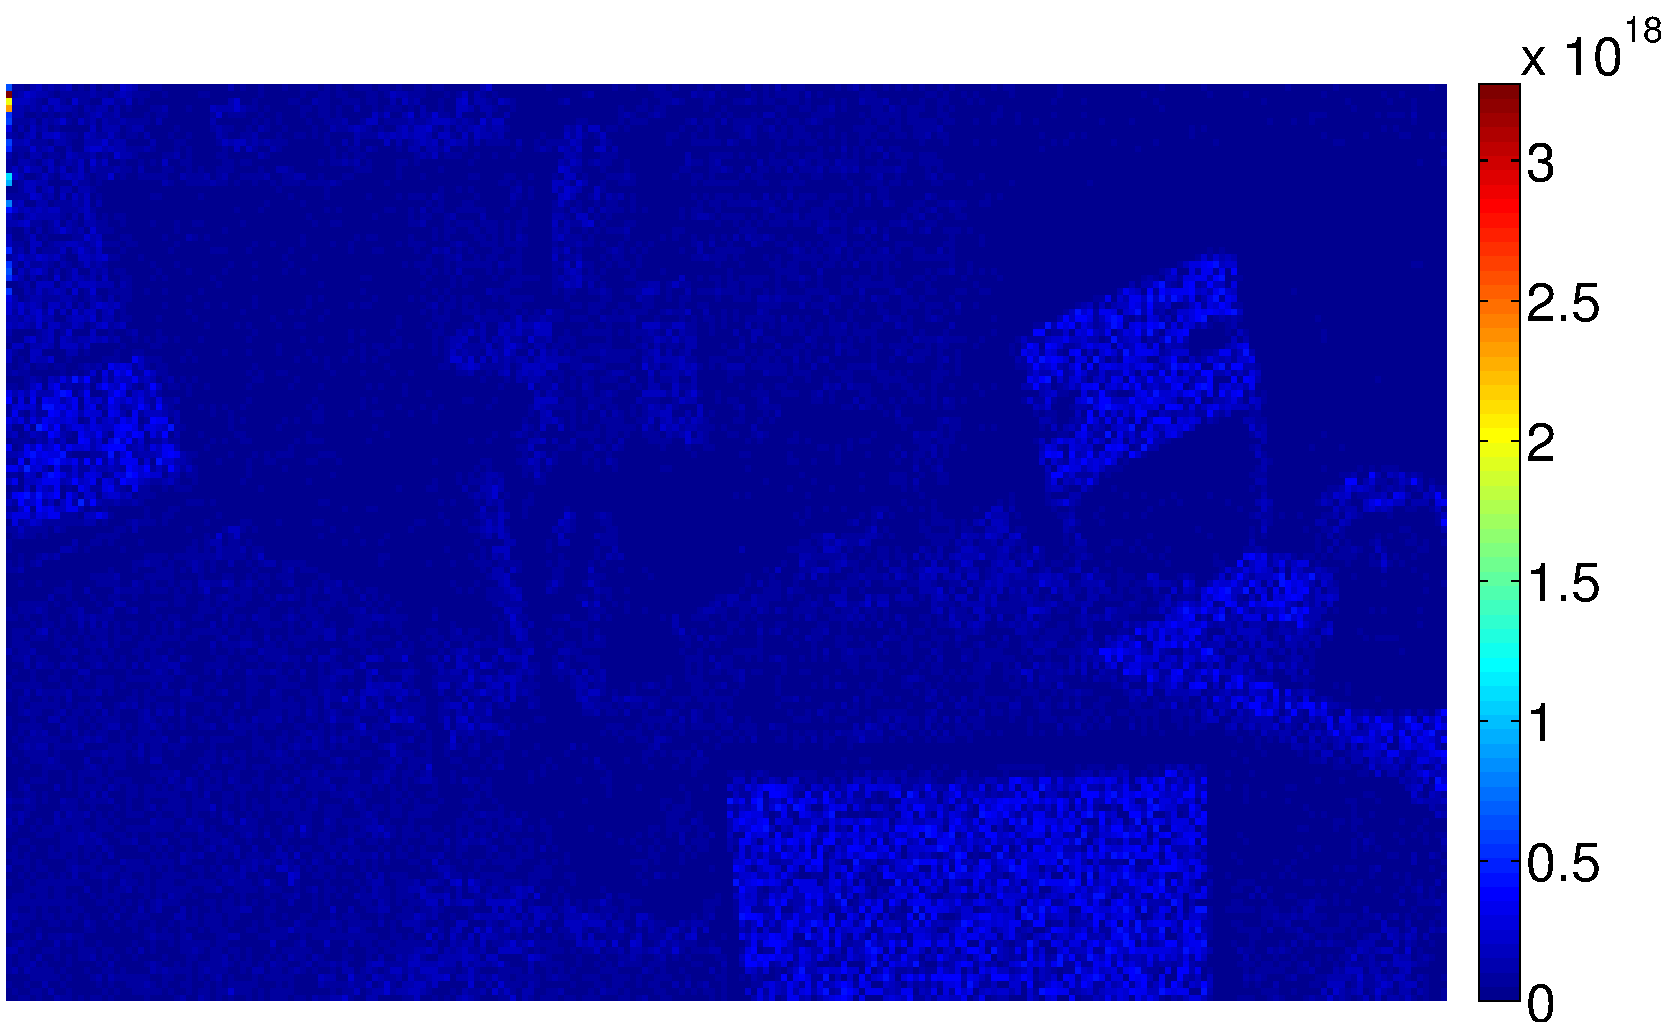
\includegraphics[width=0.3\textwidth]{chpt10_mcca/figs/mcca_ur1.pdf}
    }
    \subfigure[MCCA Left $x^{(2)}$]{
      \label{fig:chpt10:mcca_cca_left2}
      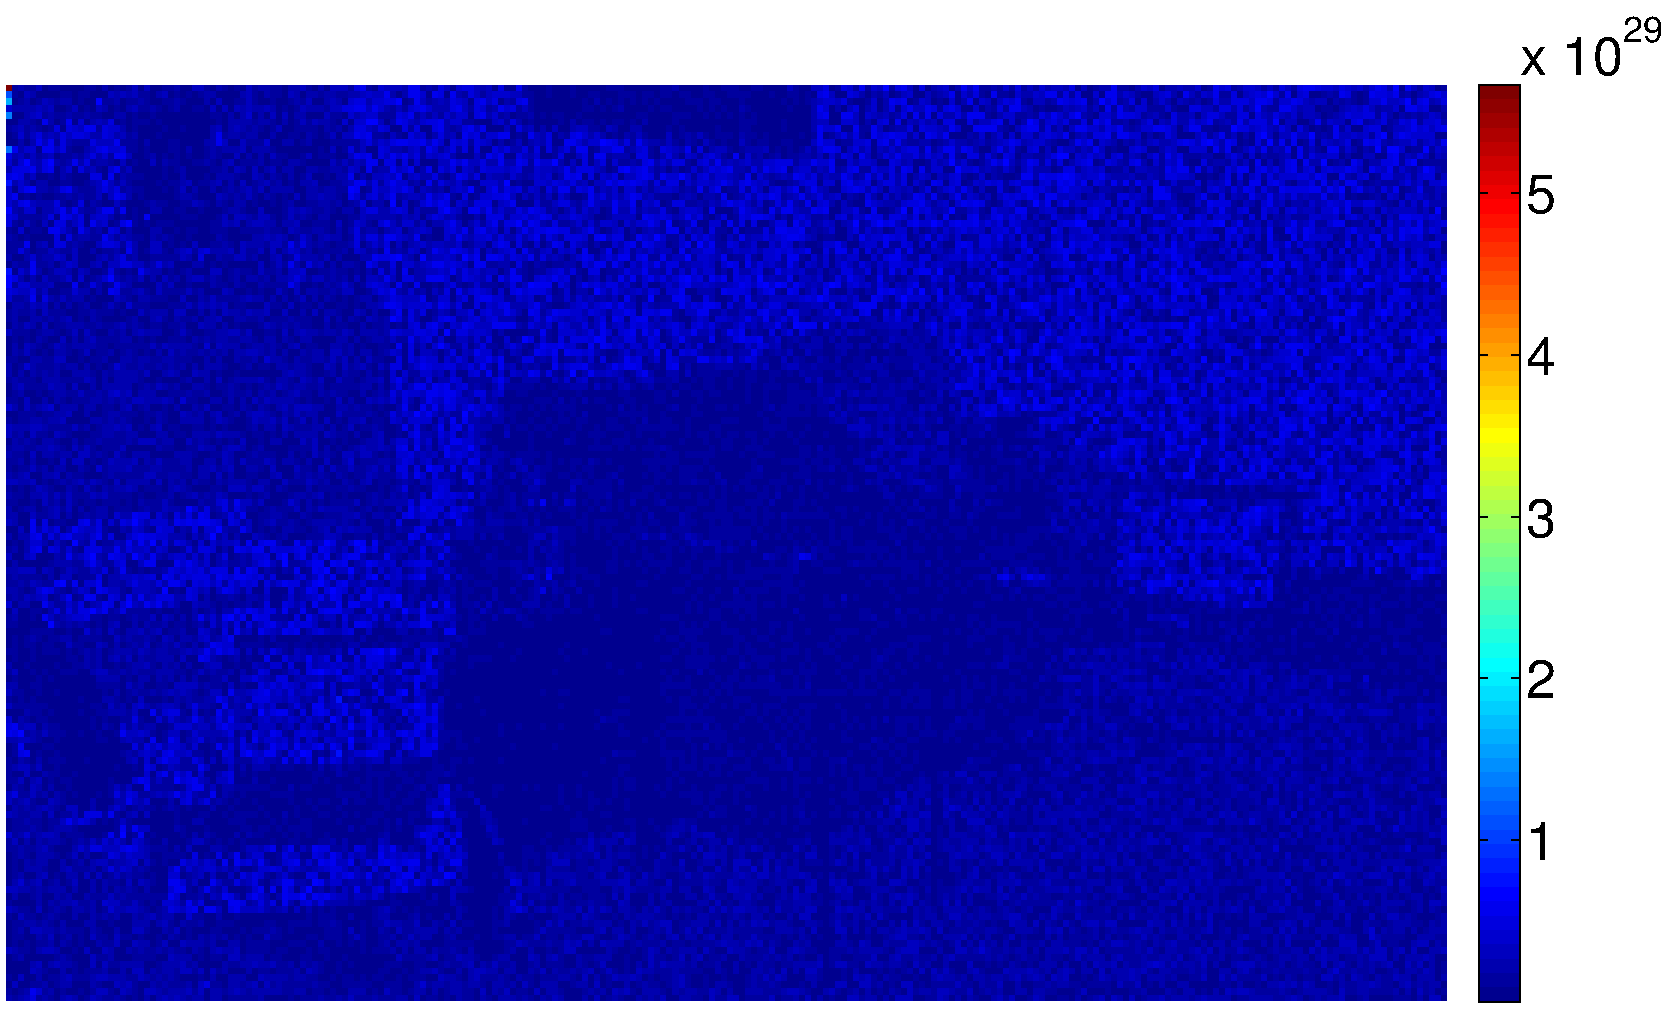
\includegraphics[width=0.3\textwidth]{chpt10_mcca/figs/mcca_ul2.pdf}
    }
    \subfigure[MCCA Middle $x^{(2)}$]{
      \label{fig:chpt10:mcca_cca_mid2}
      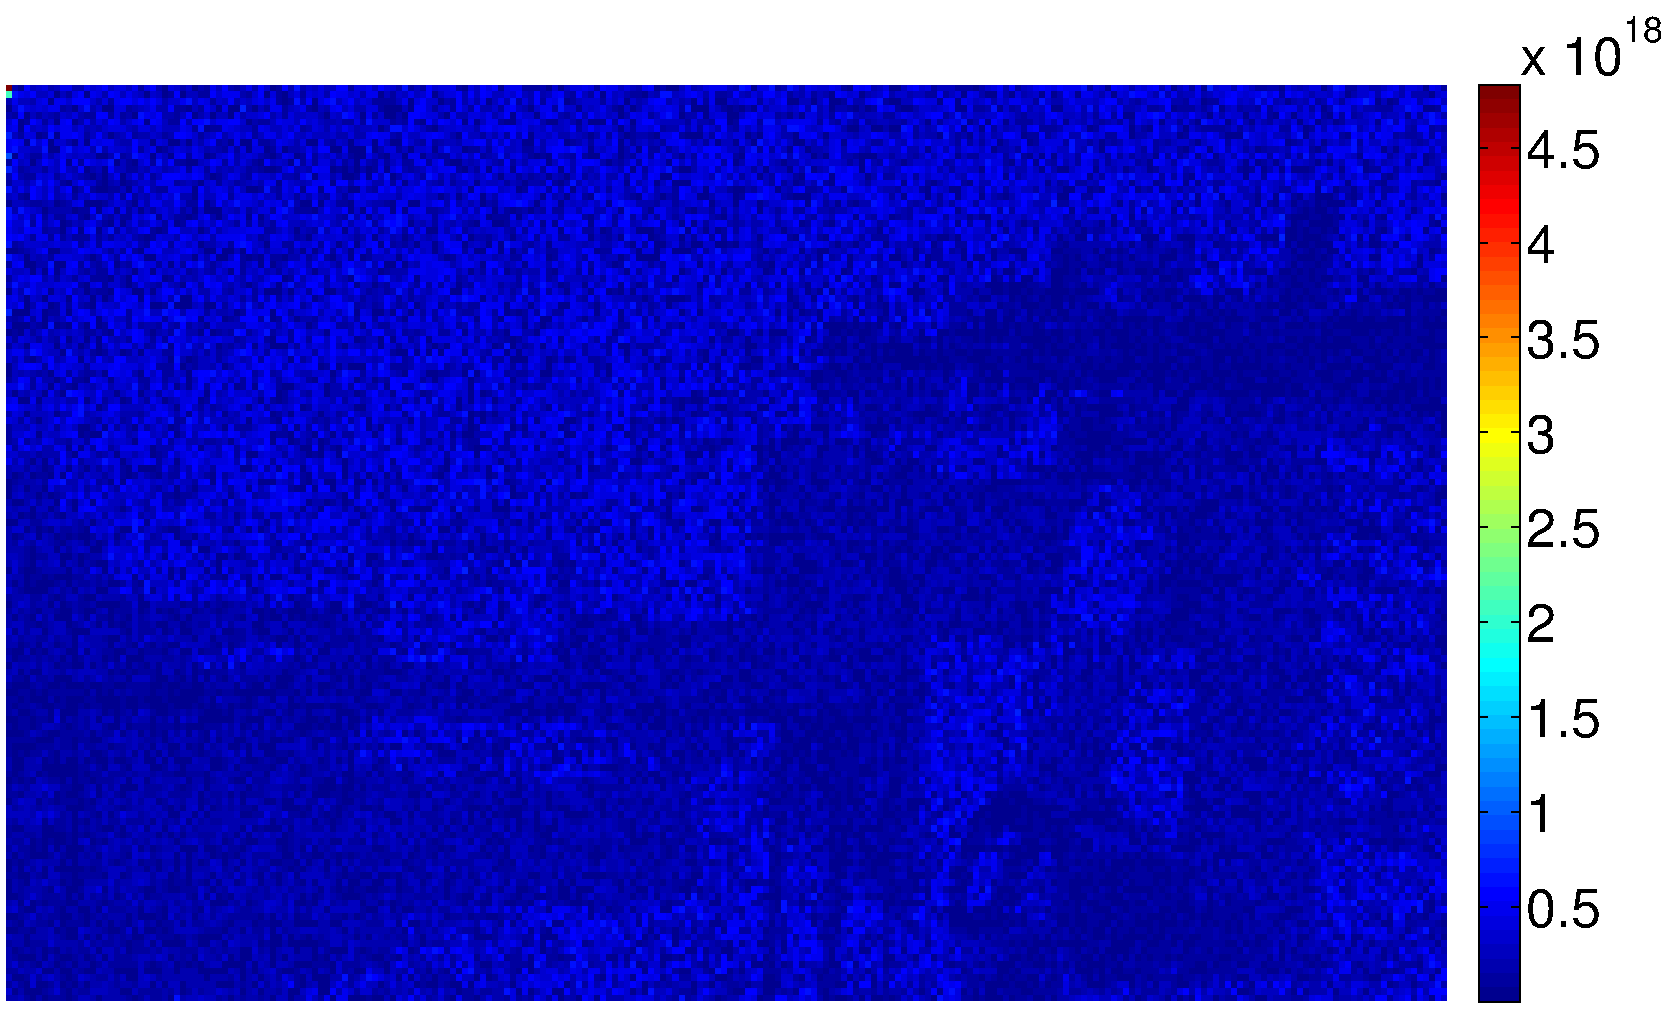
\includegraphics[width=0.3\textwidth]{chpt10_mcca/figs/mcca_um2.pdf}
    }
    \subfigure[MCCA Right $x^{(2)}$]{
      \label{fig:chpt10:mcca_cca_right2}
      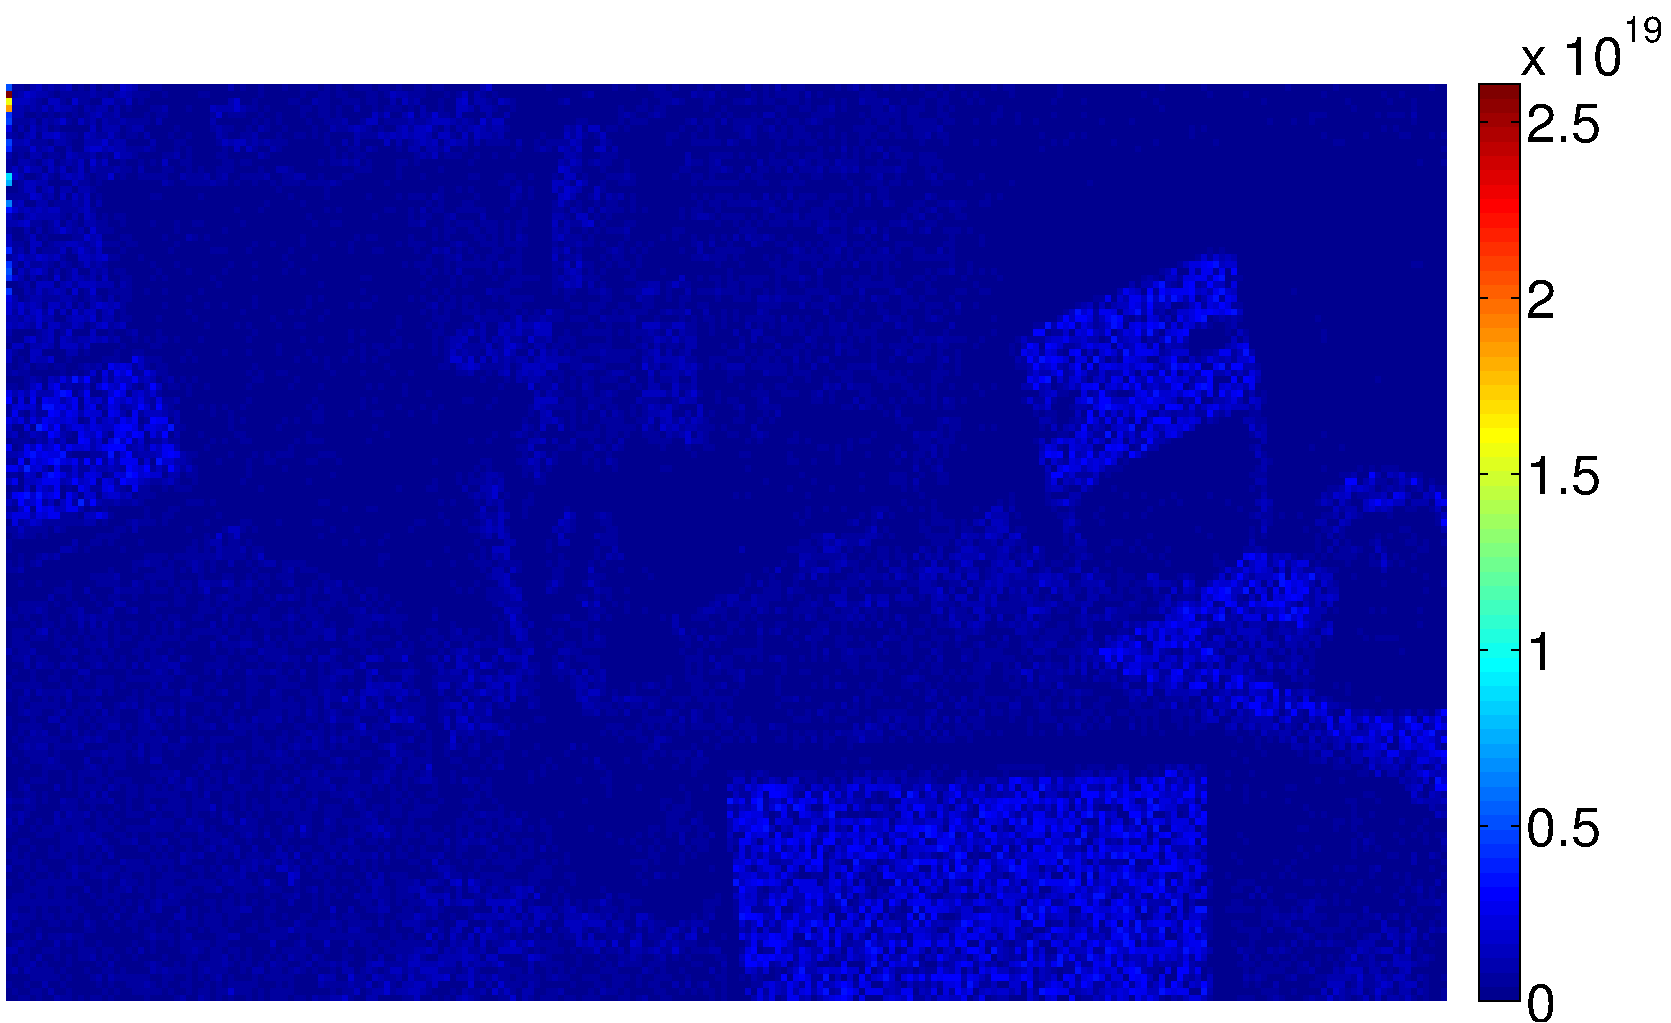
\includegraphics[width=0.3\textwidth]{chpt10_mcca/figs/mcca_ur2.pdf}
    }
    \subfigure[IMCCA Left $x^{(1)}$]{
      \label{fig:chpt10:imcca_cca_left1}
      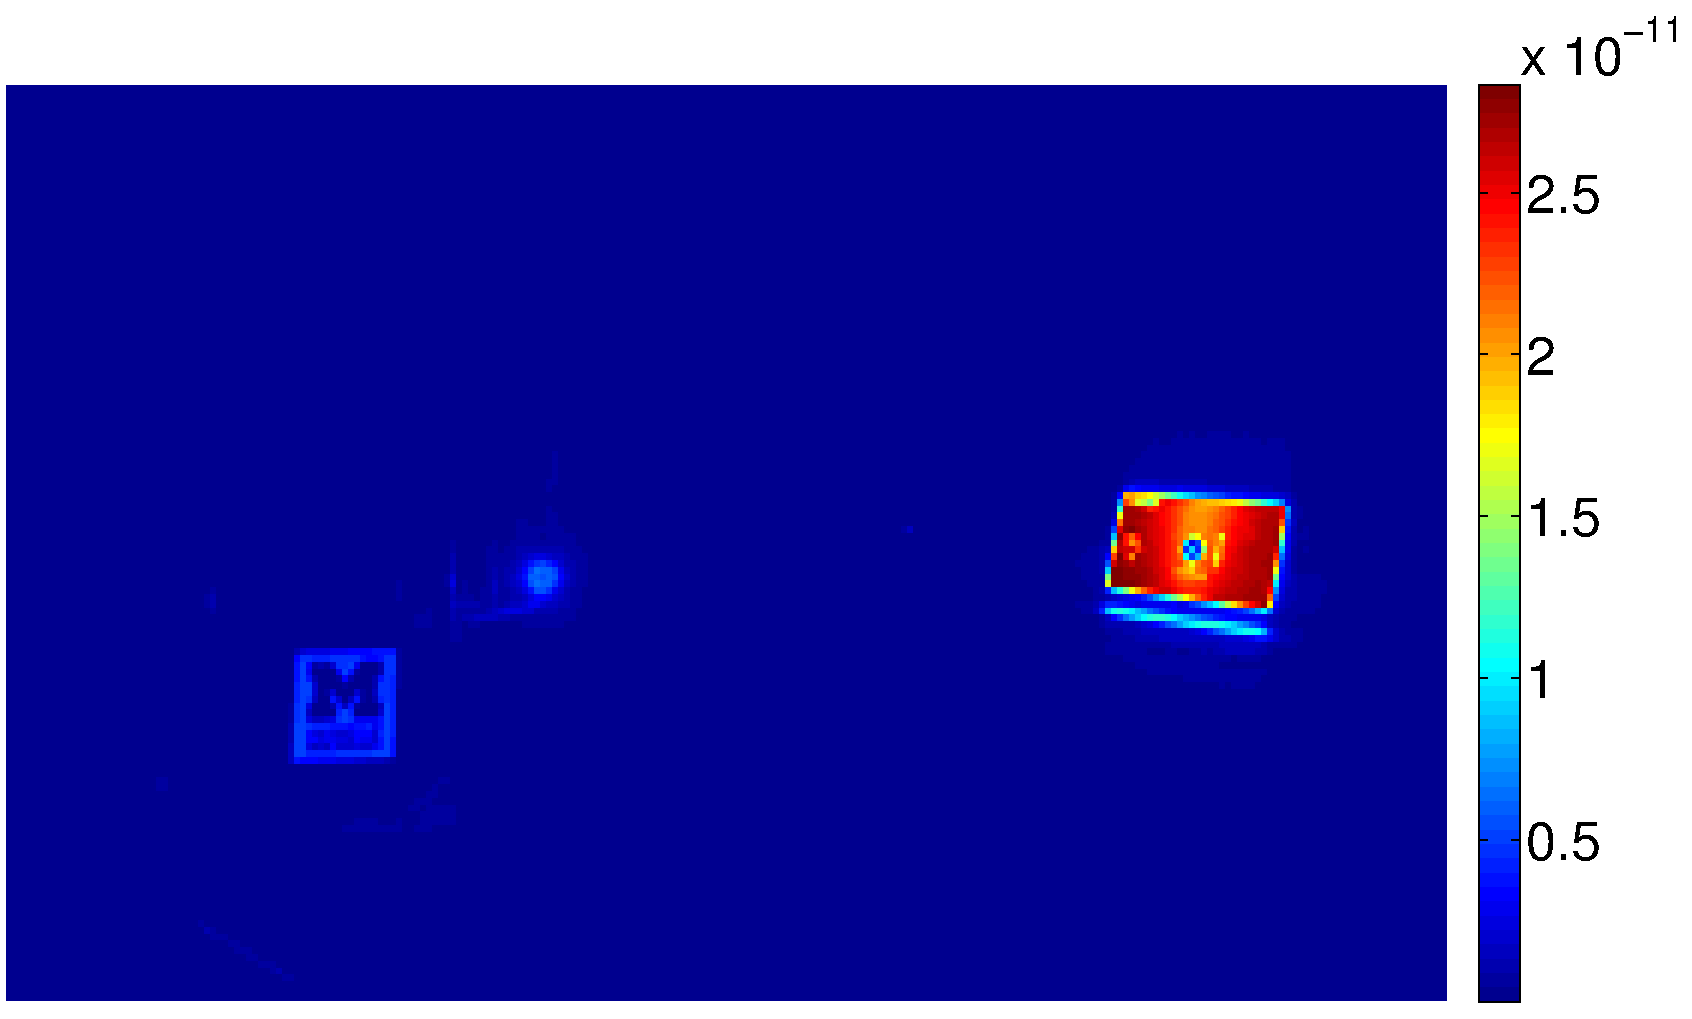
\includegraphics[width=0.3\textwidth]{chpt10_mcca/figs/imcca_ul1.pdf}
    }
    \subfigure[IMCCA Middle $x^{(1)}$]{
      \label{fig:chpt10:imcca_cca_mid1}
      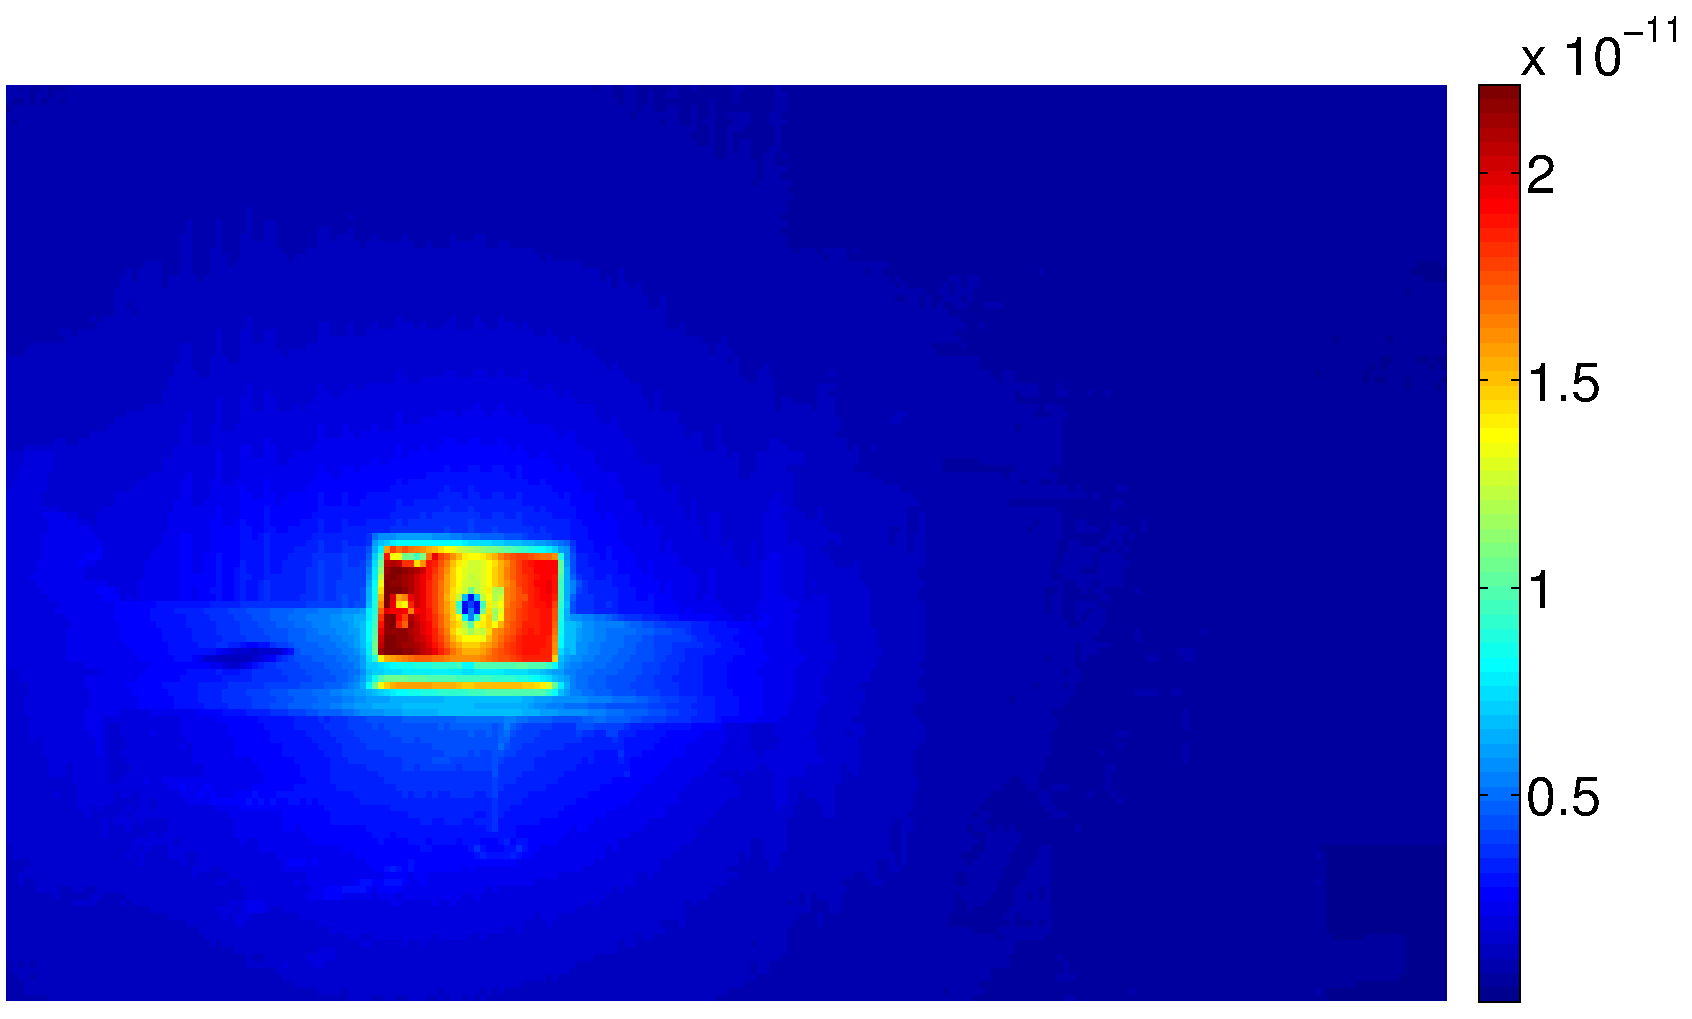
\includegraphics[width=0.3\textwidth]{chpt10_mcca/figs/imcca_um1.pdf}
    }
    \subfigure[IMCCA Right $x^{(1)}$]{
      \label{fig:chpt10:imcca_cca_right1}
      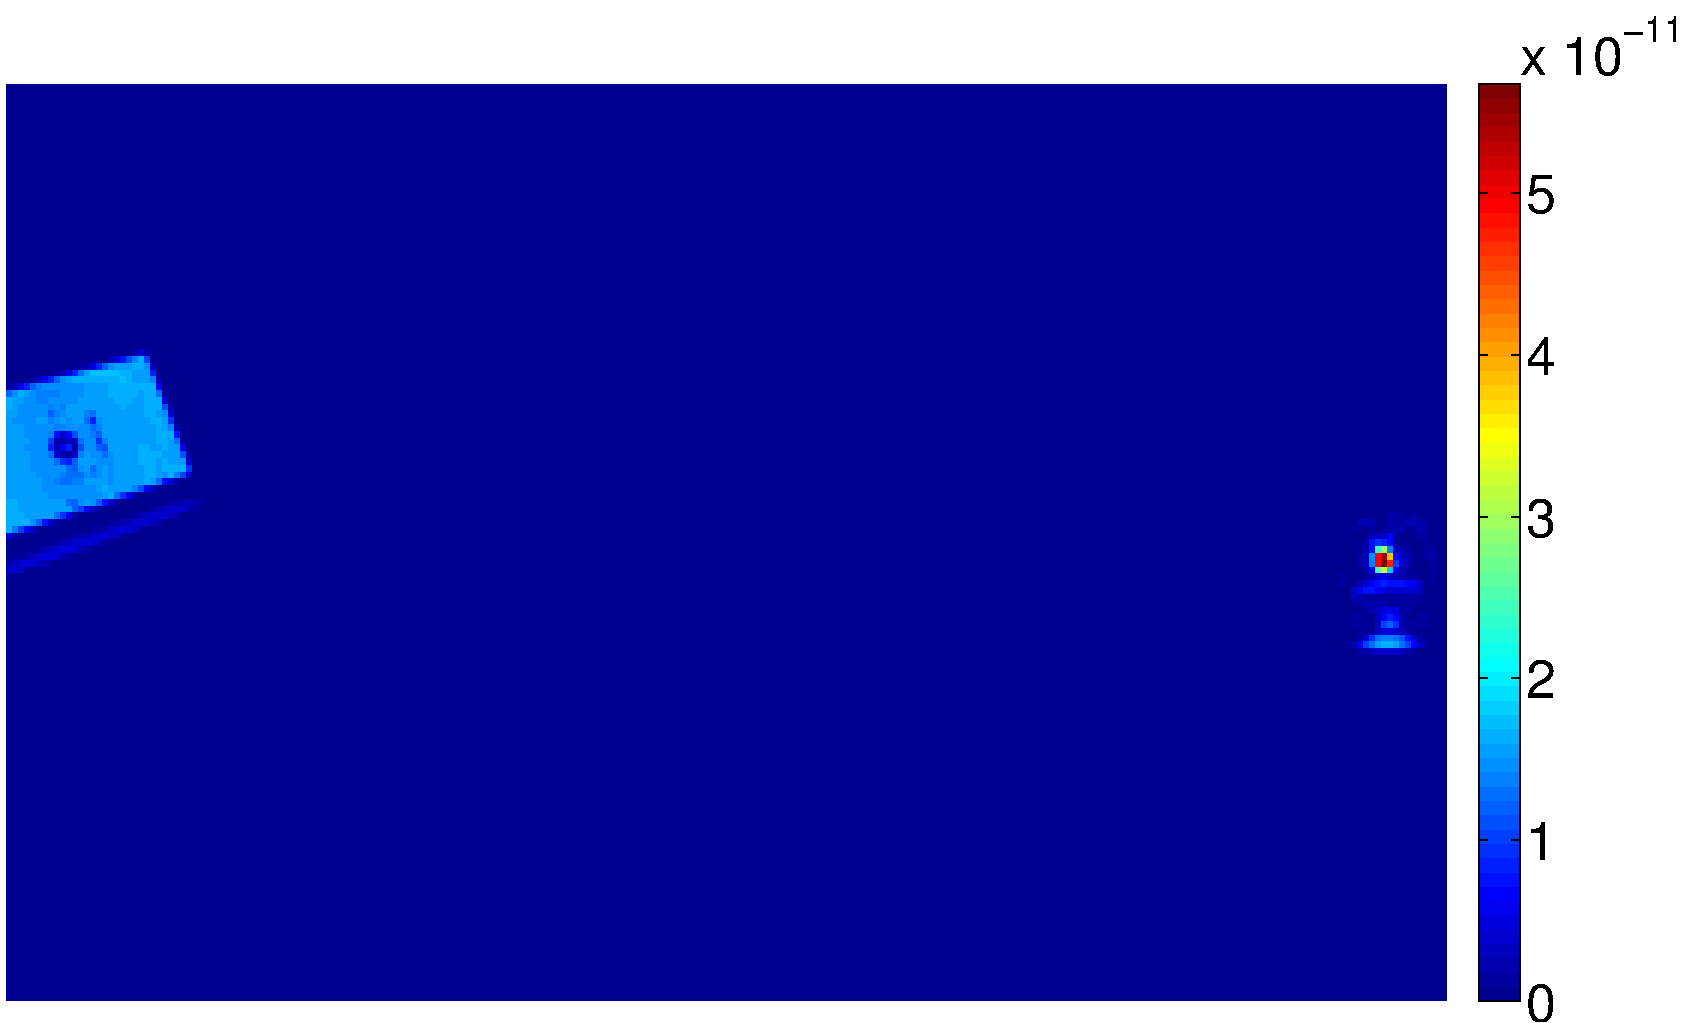
\includegraphics[width=0.3\textwidth]{chpt10_mcca/figs/imcca_ur1.pdf}
    }
    \subfigure[IMCCA Left $x^{(2)}$]{
      \label{fig:chpt10:imcca_cca_left2}
      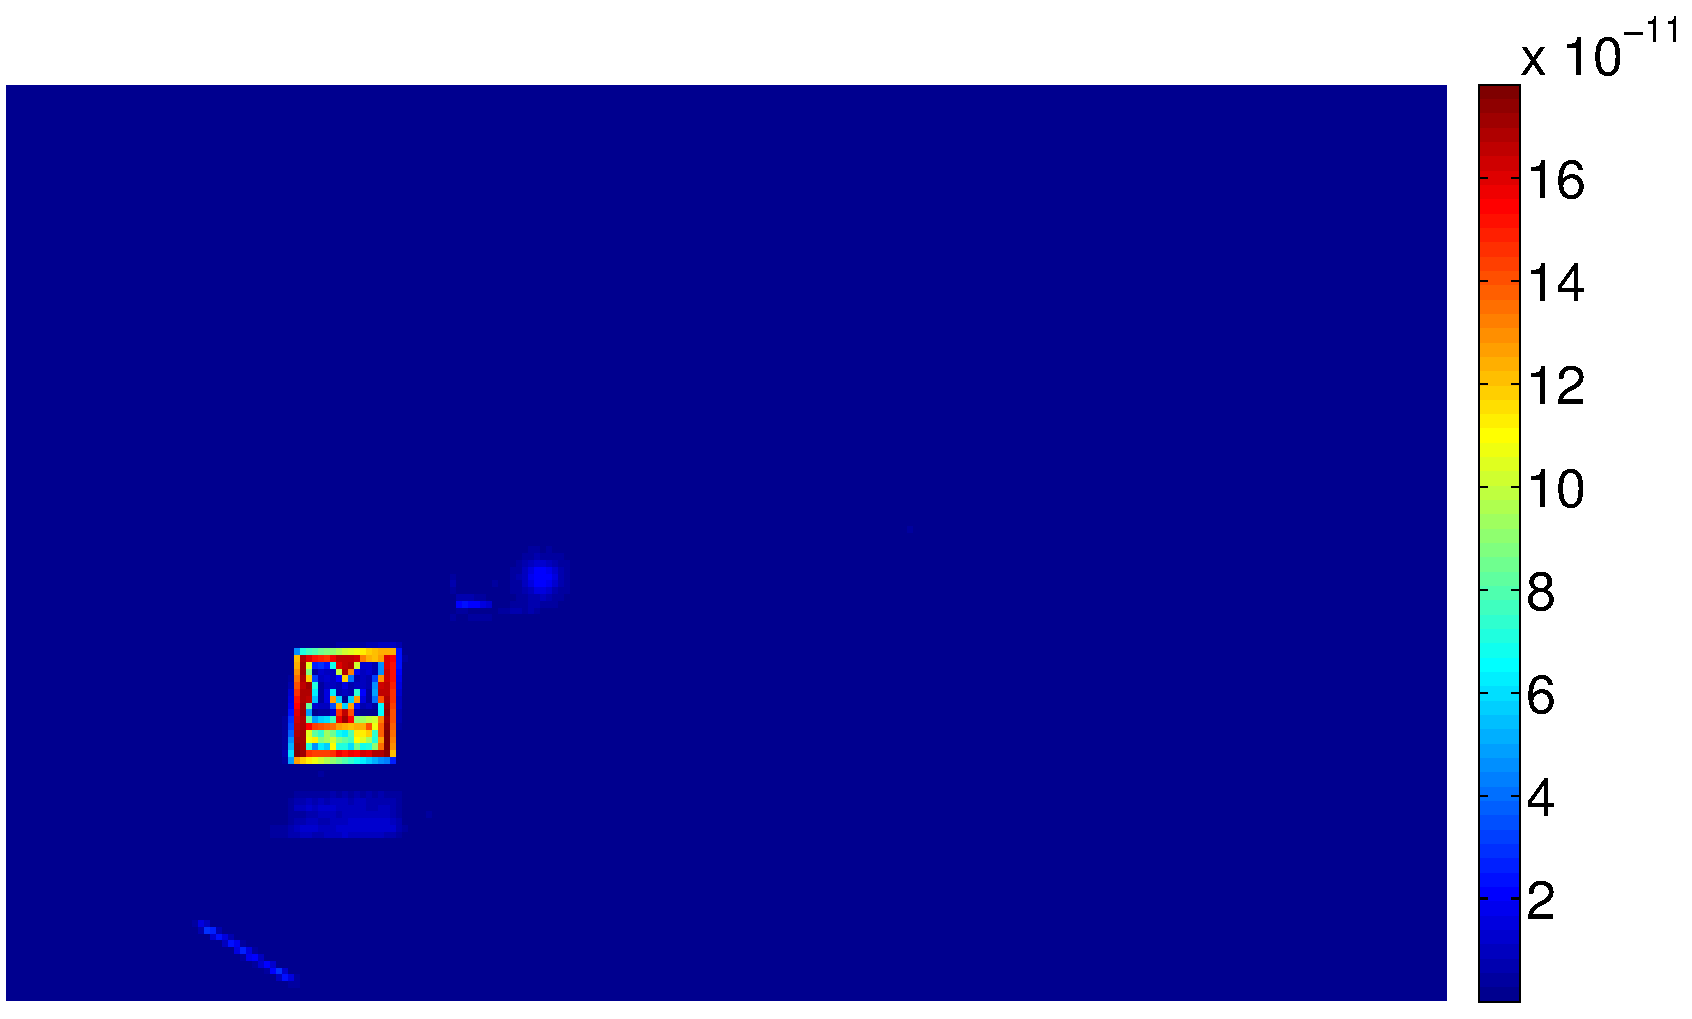
\includegraphics[width=0.3\textwidth]{chpt10_mcca/figs/imcca_ul2.pdf}
    }
    \hspace{27ex}
%    \subfigure[IMCCA Middle $x^{(2)}$]{
%      \label{fig:chpt10:imcca_cca_mid2}
%      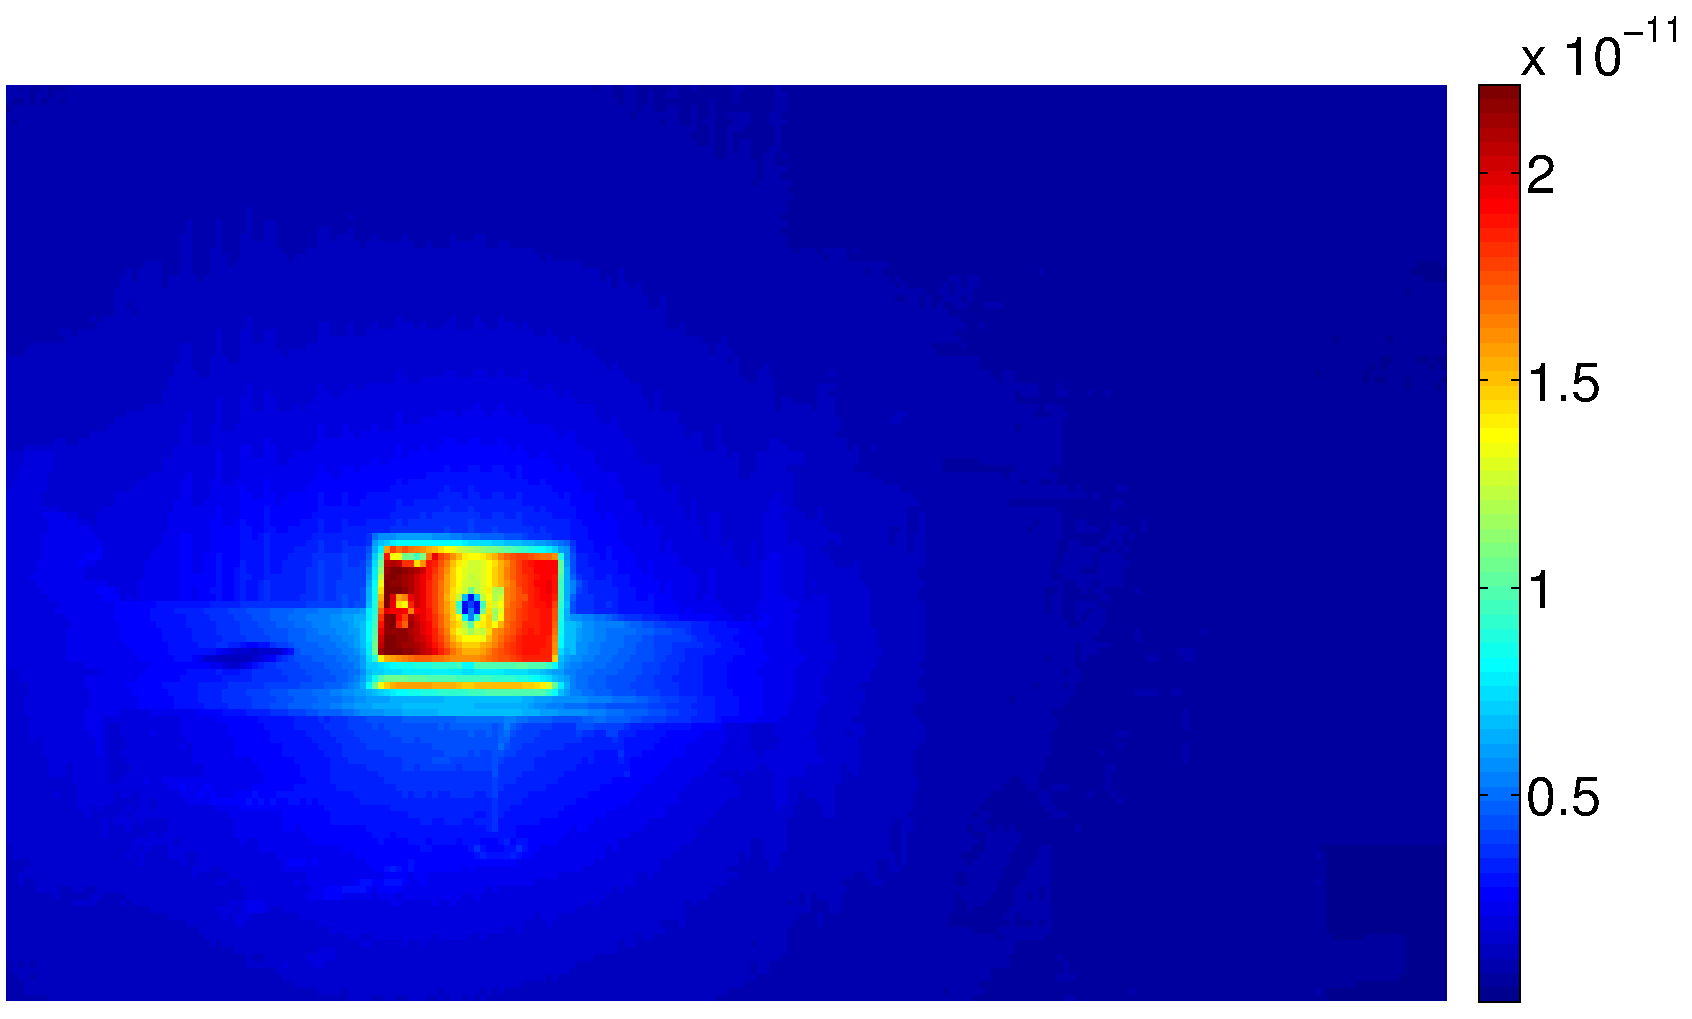
\includegraphics[width=0.3\textwidth]{chpt10_mcca/figs/imcca_um2.pdf}
%    }
    \subfigure[IMCCA Right $x^{(2)}$]{
      \label{fig:chpt10:imcca_cca_right2}
      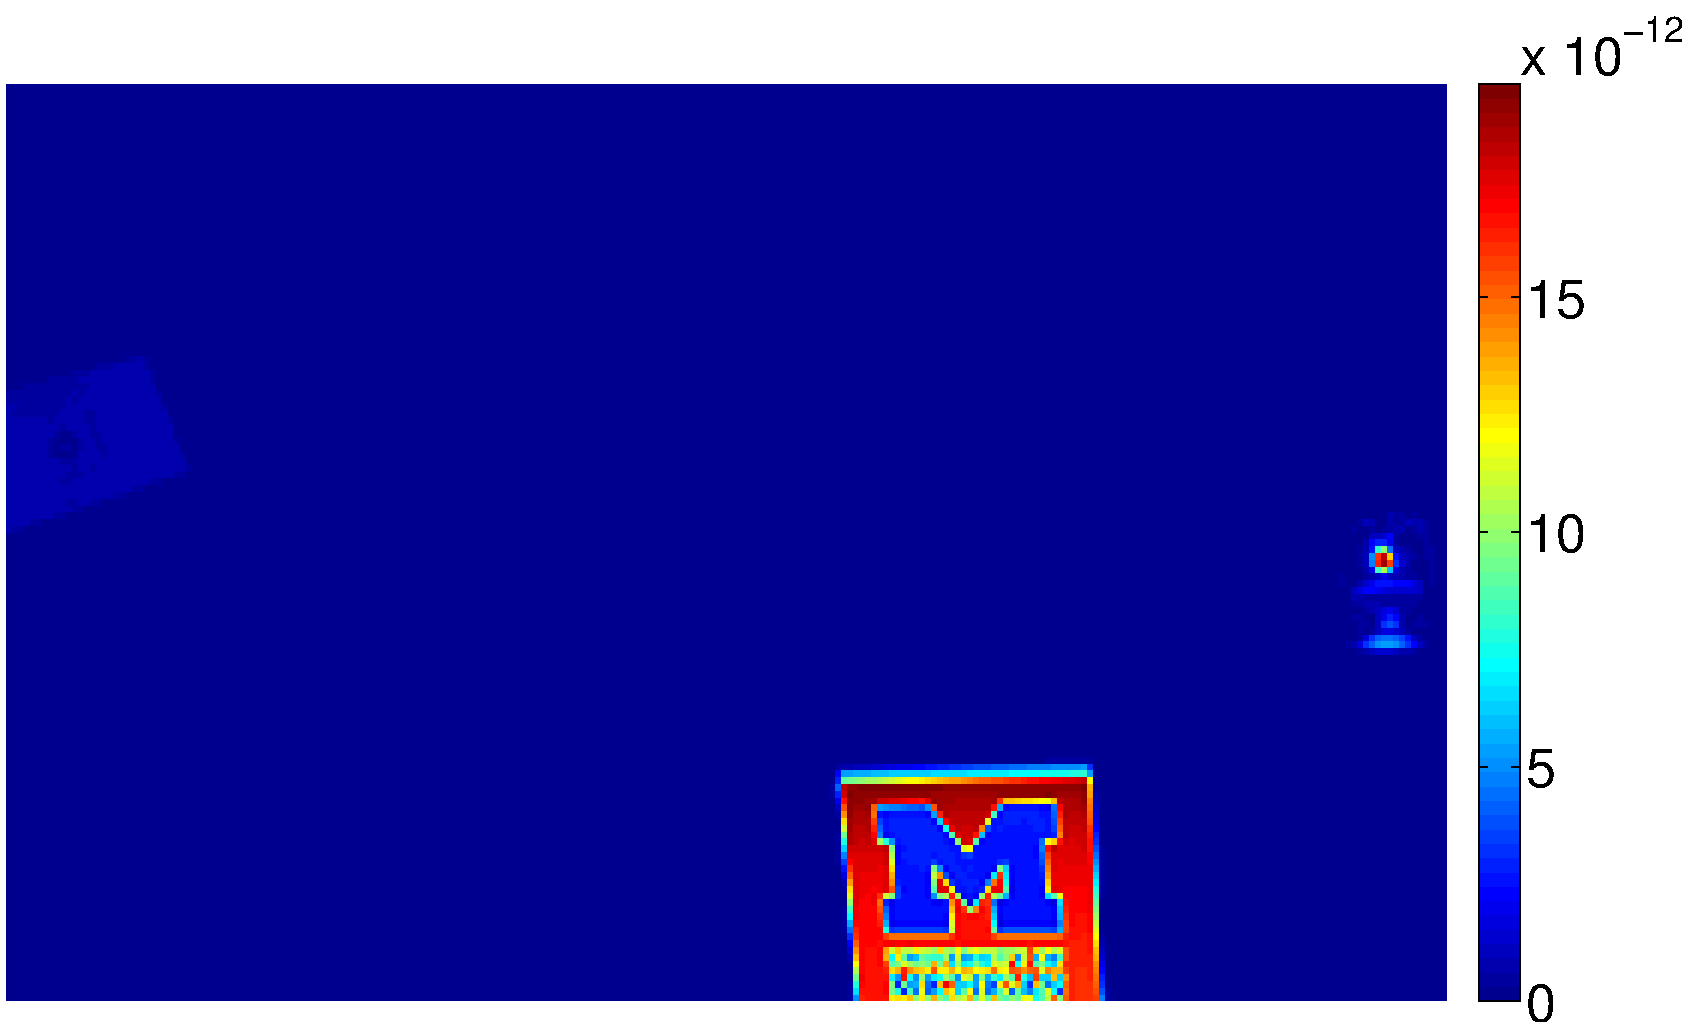
\includegraphics[width=0.3\textwidth]{chpt10_mcca/figs/imcca_ur2.pdf}
    }
    \caption{Top 2 canonical vectors for the video experiment as defined in
      (\ref{eq:chpt10:can_vect}). (a)-(c) First empirical MCCA canonical vectors. (d)-(f)
      Second empirical IMCCA canonical vectors. (g)-(i) First IMCCA canonical
      vectors. (j)-(k) Second IMCCA canonical vectors. There is no second middle camera
      IMCCA canonical vector as $\widehat{k}_{\text{middle}}=1$. Since we are in the
      sample deficient regime, empirical MCCA returns random pixels as the canonical
      vectors are random. IMCCA correctly identifies the shared light in all three views
      with the first canonical vector and the shared laptop light in the left and right
      views with second canonical vector.}
    \label{fig:chpt10:mcca_cca_vects}
  \end{center}
\end{figure*}

\section{Conclusion}

In this paper, we considered the problem of inferring, identifying and learning latent
correlations in more than two datasets.  We provided sufficient conditions for
the deterministic failure of the empirical MCCA algorithm to infer latent correlations and
showed that these will generically occur in the low-sample, high dimensional regime. We
then considered the setting where the individual datasets may be modeled as
low-rank-signal-plus-noise matrices and developed an algorithm (IMCCA) that functions well
in the low-sample, high dimensional regime. The IMCCA algorithm uses the fact that the
principal singular vectors are more informative than the other singular vectors. We
demonstrated its improved performance relative to empirical MCCA on a synthetic and real
world video dataset.
